

% DOCUMENT CLASS
\documentclass[oneside,12pt]{Classes/RoboticsLaTeX}

% USEFUL PACKAGES
% Commonly-used packages are included by default.
% Refer to section "Book - Useful packages" in the class file "Classes/RoboticsLaTeX.cls" for the complete list.
\usepackage{amsmath}
\usepackage{amsfonts}
\usepackage{algorithm}
\usepackage{algorithmic}
\usepackage[utf8]{inputenc}
\usepackage{graphicx}
\usepackage{url}% for url's in bib
\usepackage{array}
\usepackage{epstopdf}
% SPECIAL COMMANDS
% correct bad hyphenation
\hyphenation{op-tical net-works semi-conduc-tor}
%% ignore slightly overfull and underfull boxes
%\hbadness=10000
%\hfuzz=50pt
% declare commonly used operators
\DeclareMathOperator*{\argmax}{argmax}

% HEADER

\title{Algorithms for controlling and tracking UAVs in indoor scenarios}

\ifpdf
  \author{\href{mailto:andrea.nistic@gmail.com}{Andrea Nisticò \\ \vspace*{2ex}{   \     Supervised by: Marco Baglietto, Fulvio Mastrogiovanni}}
          }
  \collegeordept{\href{http://www.dibris.unige.it}{DIBRIS - Department of Computer Science, Bioengineering, Robotics and System Engineering}}
  \university{\href{http://www.unige.it}{University of Genova}}
  \crest{\includegraphics[width=35mm]{logo_unige}}
\else
  \author[Andrea Nistico']{Andrea Nistico'\\{ Supervised by: Marco Baglietto, Fulvio Mastrogiovanni}}
 %% \author{Andrea Nistico' Fulvio Mastrogiovanni}
  \collegeordept{DIBRIS - Department of Computer Science, Bioengineering, Robotics and System Engineering}
  \university{University of Genova}
  \crest{\includegraphics[width=30mm]{logo_unige}}
\fi

% DECLARATION
% Use the following command to change the declaration text:
%\renewcommand{\submittedtext}{INSERT NEW TEXT HERE}
\degree{Robotics engineering}
\degreedate{September 18, 2015}

%%%%%%%%%%%%%%%%%%%%%%%%%%%%%%%%%%%%%%%%%%%%%%%%%%%%%%%%%%%%%%%%%%%%%%%%%%%%%%%%

\begin{document}

% A page with the abstract and running title and author etc may be
% required to be handed in separately. If this is not so, comment
% the following 3 lines:
% \begin{abstractseparate}
%   %%%%%%%%%%%%%%%%%%%%%%%%%%%%%%%%%%%%%%%%%%%%%%%%%%%%%%%%%%%%%%%%%%%%%%%%%%%%%%%%
%2345678901234567890123456789012345678901234567890123456789012345678901234567890
%        1         2         3         4         5         6         7         8
% THESIS ABSTRACT

% Use the following style if the abstract is long:
%\begin{abstractslong}
%\end{abstractslong}

\begin{abstracts}

Quadcopter, also known as quadrotor, is a helicopter with four rotors. The rotors are directed upwards and they are placed in a square formation with equal distance from the center of mass of the quadcopter. The quadcopter is controlled by adjusting the angular velocities of the rotors which are drived by electric motors. An on board autopilot, namely PiXHawk with PX4 software, pack all the interfaces for sensors, motor controllers and radio antennas. It also manage the control, state estimation and signals processing. The goal of this master thesis is to develop algorithms for UAV trajectory planning and execution (as well as the related SW components), using the motion capture system as the source of the UAV position feedback. An IRIS quadrotor it is used form 3d Robotics. After an introduction to the components, the integration between them both hardware and software is presented. The model of the IRIS is briefly derived and explained as well as the control techniques involved in the open source autopilot. Moreover a software architecture is presented where a task based program is able to read a set of tasks from a list and let the robot execute them sending position set point through radio link. At the end an algorithm for tracking and landing on a mobile platform is explained and the overall results are presented.

\end{abstracts}
% \end{abstractseparate}

\maketitle

% add an empty page after title page
\newpage\null\thispagestyle{empty}\newpage

% set the number of sectioning levels that get number and appear in the contents
\setcounter{secnumdepth}{3}
\setcounter{tocdepth}{3}

\frontmatter

%%%%%%%%%%%%%%%%%%%%%%%%%%%%%%%%%%%%%%%%%%%%%%%%%%%%%%%%%%%%%%%%%%%%%%%%%%%%%%%%
%2345678901234567890123456789012345678901234567890123456789012345678901234567890
%        1         2         3         4         5         6         7         8
% THESIS ACKNOWLEDGEMENTS

% Use the following style if the acknowledgements are long:
%\begin{acknowledgementslong}
%\end{acknowledgmentslong}

\begin{acknowledgements}


I would like to express my deepest gratitude to my supervisor, Prof. Marco Baglietto, for his patience, caring, guiding and mentoring. His guidance helped me since the beginning of this work. I also would like to thank him for the enormous patience he had and the dose of sarcasm added o each conversation. 

I would like to thank my second supervisor, Prof. Fulvio Mastrogiovanni, for his big help, huge encouragement and for always bringing a good laugh among us. 

I would like to express my gratitude to my co-supervisor Tommaso Falchi Delitalia, who helped me so much especially in the beginning of the work. He is the one who made this thesis possible and moreover, the one who let me discover the wonderful world of aerial robotics.

I would like to express my deepest gratitude to the entire EMARO staff, to the professors who supported me and thought many interest things. Special thanks to Gaetan Garcia, the funny man who thought me robotics. 

Sincere gratitude to my colleagues and friends who gave me always the support needed. In particular Alessio Capitanelli who started a beautiful journey with me five years ago. Thanks to my lab fellow Luca Buoncompagni who helped me in many ways in the most difficult moments.

I express my gratitude to my girlfriend Laura, who begun this adventure with me two years ago and continuously supports me.
 
Finally, I take this opportunity to express the profound gratitude from my deep heart to my beloved parents, for the enormous support they gave me since the beginning of my life.

Any future success that I may accomplish will be caused by those mentioned above, thank you.
  


\end{acknowledgements}
\include{Dedication/dedication}
%%%%%%%%%%%%%%%%%%%%%%%%%%%%%%%%%%%%%%%%%%%%%%%%%%%%%%%%%%%%%%%%%%%%%%%%%%%%%%%%
%2345678901234567890123456789012345678901234567890123456789012345678901234567890
%        1         2         3         4         5         6         7         8
% THESIS ABSTRACT

% Use the following style if the abstract is long:
%\begin{abstractslong}
%\end{abstractslong}

\begin{abstracts}

Quadcopter, also known as quadrotor, is a helicopter with four rotors. The rotors are directed upwards and they are placed in a square formation with equal distance from the center of mass of the quadcopter. The quadcopter is controlled by adjusting the angular velocities of the rotors which are drived by electric motors. An on board autopilot, namely PiXHawk with PX4 software, pack all the interfaces for sensors, motor controllers and radio antennas. It also manage the control, state estimation and signals processing. The goal of this master thesis is to develop algorithms for UAV trajectory planning and execution (as well as the related SW components), using the motion capture system as the source of the UAV position feedback. An IRIS quadrotor it is used form 3d Robotics. After an introduction to the components, the integration between them both hardware and software is presented. The model of the IRIS is briefly derived and explained as well as the control techniques involved in the open source autopilot. Moreover a software architecture is presented where a task based program is able to read a set of tasks from a list and let the robot execute them sending position set point through radio link. At the end an algorithm for tracking and landing on a mobile platform is explained and the overall results are presented.

\end{abstracts}
\tableofcontents
\listoffigures

%\printglossary  % Print the nomenclature (WAY TOO COMPLEX FOR ME NOW!)
%\addcontentsline{toc}{chapter}{Nomenclature}

\mainmatter

% THESIS INTRODUCTION

\chapter{Introduction}
\label{chap:introduction}
\ifpdf
    \graphicspath{{Introduction/Figures/PNG/}{Introduction/Figures/PDF/}{Introduction/Figures/}}
\else
    \graphicspath{{Introduction/Figures/EPS/}{Introduction/Figures/}}
\fi

% short summary of the chapter
\section*{Summary}

This Chapter will introduce  the reader to the topic of this master thesis. It will present the problem statement and the followed work plan.

\section{Overview}

In the latest years, aerial robotics has grown so fast both in technology and popularity among the public and multirotor aircrafts such as quadcopters are one of the most promising fields. In fact those type of vehicles have become a standard platform for research in many laboratories , driven by totally different customer needs the research improved substantially. They have sufficient payload and flight endurance to support a number of indoor and outdoor applications, and the improvements of battery and other technology is rapidly increasing the scope for commercial opportunities. They are highly maneuverable and enable safe and low-cost experimentation in mapping, navigation, and control strategies for robots that move in three-dimensional space. Small quadrotors have been demonstrated for exploring and mapping 3-D environments; transporting, manipulating, and assembling objects; and acrobatic tricks such as juggling, balancing, and flips. \\*

\begin{figure}[h]
\centering
 \noindent
 \includegraphics[width=0.4\textwidth]{amazon.jpg}\hspace{0.1\textwidth}
 \includegraphics[width=0.4\textwidth]{police-drone.jpg}\\[2em]
 \includegraphics[width=0.4\textwidth]{gopro.jpg}\hspace{0.1\textwidth}
 \includegraphics[width=0.4\textwidth]{microcopter.jpg}\par
 \caption{Different applications of multirotors}
 \label{figure:applications}
\end{figure}

\noindent
As stated before, the uses of this platform are many and limited
only by the imagination of the designers. Figure \ref{figure:applications} illustrates various application going from search and rescue to public defense, most of them in outdoor scenarios. Very interesting is to investigate the possible use of this technology in an indoor scene where the comforting signal of the GPS is not present and analyze every aspect of flight going from state estimation, control and stability to autonomy, path planning and high level automation. \\*

This work investigates the integration between different heterogeneous entities as well as the possibility to design a safe, reliable and flexible architecture capable of letting the robot navigate safely in an indoor environment. At the end a simple algorithm for landing on a mobile platform is presented with very interesting results demonstrating the potential of this setup.

\subsection{Hosting laboratories}
This thesis is carried out as a cooperation between the Laboratorium Lab (focus:
autonomous robotics and ambient intelligence), the NOCC Lab (focus: control,
identification and estimation) and the EMARO@DIBRIS Lab.

\newpage

\section{Problem statement}

The goal of this master thesis to develop algorithms for UAV trajectory planning and execution (as well as the related SW components), using the motion capture system as the source of the UAV position feedback. Once achieved stability more complex aspects are investigated, a task based software architecture is presented and a simple technique for landing on a mobile platform is proposed.
The above stated, is formulated in to the following problem statement for the project: \\*

\noindent
\textit{We want to design a set of algorithms and SW components enabling a quadrotor to achieve stability, through position feedback given from a motion capture system, and perform different tasks in an indoor scenario. }

\subsection{Work plan}
The work got through several tasks covering all aspects, they can be distinctly divided in main blocks hence defining the work plan.

\begin{enumerate}

\item Analysis of state of the art approaches to UAV control, modeling, trajectory planning and execution

\item Technical analysis and documentation on the given tools (Autopilot, Motion Capture, IRIS Quadcopter)

\item Integration between mocap and IRIS
\begin{itemize}

\item Integration and testing between mocap and onboard estimation modules
\item Integration and testing of onboard controller through set point control

\end{itemize}

\item Design of the high level software architecture 
\item Testing the software, coding and debugging different kind of tasks
\item Design and testing an algorithm for landing on a mobile platform

\end{enumerate}

\subsection{Thesis structure}
The thesis presents procedures, techniques, comments and results obtained during the work. The document is divided in chapters dedicated to particular aspects of the project, the structure is the following: 

\paragraph{Chapter 2} Synthesizes the preliminary literature review explaining existing research, products and systems and analyzes some robotics platforms and tools. A suitable modeling technique for this kind of vehicles is described introducing additional non linearities and explaining when the model uses them.
Moreover it introduces a survey on various control techniques that are currently used highlighting pros and cons. At the end some comments are given about software architecture trends which are used in this field. 


\paragraph{Chapter 3}

This chapter introduces the reader the current laboratory setup illustrating which kind of tools are used as well as the specifications of each component. Then it presents the integration both at hardware and software levels of each part of the system. 

\paragraph{Chapter 4}
This part concerns the modeling of the IRIS quad rotor. A model of the quadrotor is necessary to develop a controller and understand better its dynamics. The first part presents some generalities including the reference frames used in order to define the world and the robot. It also contains a list of assumptions done to simplify the model. After, the involved physical principles and the actual derivation of the model are explained.

\paragraph{Chapter 5}

This chapter presents the techniques that are used to estimate the system's states and to stabilize the IRIS robot which are currently implemented in the PX4 Firmware. After a quick overview of the estimator modules, the controller architecture is presented. Moreover, this chapter explains in details how the on board autopilot interfaces with the software architecture and which modules are involved.

\paragraph{Chapter 6}

This Chapter introduces the reader to the software architecture running off board on Linux. The introduction presents a  general overview on software architectures, expresses the needs of such a system and in particular it describes the environment and software tools involved. Next section presents the design pattern according to which the software is organized explaining its advantages and limitations. Then the software components are described with more detail one by one and the results of the experiments are reported. 


\paragraph{Chapter 7}

This chapter concerns with the task of landing on a platform of arbitrary height while it is moving on the horizontal plane. After a brief introduction to the topic and the statement of general assumptions, the experimental setup is described. Later on the solution to the problem is presented and the control algorithm described. Last section presents and comments experiment results.

\paragraph{Chapter 8}

The last chapter presents the conclusions of this work. It highlights the most relevant steps and summarizes what has been done. Then it points out what could be improved and gives a number of ideas relating the future work.












% THESIS CHAPTER

\chapter{Related work}
\label{chap:second
}
\ifpdf
    \graphicspath{{Chapter2/Figures/PNG/}{Chapter2/Figures/PDF/}{Chapter2/Figures/}}
\else
    \graphicspath{{Chapter2/Figures/EPS/}{Chapter2/Figures/}}
\fi

% short summary of the chapter
\section*{Summary}
This chapter synthesizes the preliminary literature review explaining existing research, products end systems. It analyzes some robotics platforms and tools, in particular presents an overview of existing autopilots boards and software as well. A suitable modeling technique for this kind of vehicles is described introducing additional non linearities and explaining when the model uses them.\\*
Moreover it introduces a survey on various control techniques that are currently used showing pros an cons. \\*
At the end some comments are given about software architecture trends which are used in this field. 

\section{Quadrotor platform}

Flying objects have always exerted a great fascination on man encouraging all kinds of research and development. This intrigue for reaching the sky took all the form of imagination such as myths and legends. Many different and bizarre machines were theorized but very interesting were the precursors of the helicopter. Few visionaries, such as Leonardo da Vinci in the late 15th Century, foresaw an aerial application in the widely used windmill \cite{Heli} coming up with the famous screw design as propeller. Even if it never worked, Leonardo's design was very innovative and this challenge has generated centuries of frustration and hundreds of dramatic attempts without being fade. Only in 1933 Juan de la Cierva gave us the autogiro. The first pratical rotocraft invented which led to what we usually call helicopter. \par Few years after the first manned plane was invented, Dr. Cooper and Elmer Sperry designed the automatic gyroscopic stabilizer \cite{gyro}, which helps to keep an aircraft flying straight and level. This was the kick of unmanned vehicle research which has its starting point back to WWI and WWII. Few years after, sofisticated machines are seen in battle fields such as the famous Predator by General Atomics, the Hammeread by Piaggio Aerospace or the Pioneer by Israel Aerospace Industries. 
\begin{figure}[h]
\centering
 \includegraphics[width=0.7\textwidth]{predator.jpg}
 \caption[Predator UAV]{Predator Unmanned Aerial Vehicle }
 \label{figure:predator}
\end{figure}

\noindent
In the last ten years technology has taken a giant leap forward and the concept on Micro Aerial Vehicle (MAV) was born. Mavs are a class of UAVs with the feature of being relatively small and may be autonomous. Development is driven by commercial, research, government, and military purpose. The small craft allows remote observation of hazardous environments inaccessible to ground vehicles. MAVs have been built also for hobby purposes, such as aerial robotics contests and aerial photography.\par The union of Micro Aerial technology and the helicopter concept brings the quadrotor platform. Quadcopter, also known as quadrotor, is a helicopter with four rotors. The rotors are directed upwards and they are placed in a square formation with equal distance from the center of mass. The quadcopter is controlled by adjusting the angular velocities of the rotors which are spun by electric motors.\par Designers came up with different projects and the market is now full of different vendors. The standard platform is the four propeller shape but
\begin{table}[h]
  \centering
  \begin{tabular}{ | c | m{5cm} | m{5cm} | }
    \hline
    Image & Description & Designer \\ \hline
   \parbox[c]{4cm}{
   \vspace{1ex}
      \includegraphics[width=\linewidth ]{Asctec_Falcon.jpg}
    }
    &
    \textbf{Falcon 8}, used by professionals for mapping and inspections.
    & 
   Produced by Ascending Technologies \cite{Ascend}
    \\ \hline
     \parbox[c]{4cm}{
      \includegraphics[width=\linewidth]{phantom.jpg}
   }
    & \textbf{Phantom 3}, ready to use high quality commercial platform.
    & Produced by DJI \cite{DJI}.
    \\ \hline
    \parbox[c]{4cm}{
      \includegraphics[width=\linewidth]{parrot.jpg}
   }
    & \textbf{AR.Drone}, ready to fly and cheap.
    & Produced by Parrot \cite{ARDrone}.
    \\ \hline 
     \parbox[c]{4cm}{
      \includegraphics[width=\linewidth]{special_one.jpg}
   }
    & \textbf{Flamewheel}, this kit must be assembled by the user. Good quality.
    & Produced by DJI \cite{DJI} and assembled by Lorenz Meier \cite{Flamewheel} from PixHawk team.
    \\ \hline 
    \parbox[c]{4cm}{
      \includegraphics[width=\linewidth]{iri.jpg}
   }
    & \textbf{IRIS}, almost ready to use. High quality and robust but relatively cheap.
    & Produced by 3D Robotics \cite{3Dr}.
    \\ \hline 
    
      \end{tabular}
  \caption{Some copters designs}\label{tab:copters}
\end{table}
the architecture can be eventually expanded, with advantages and drawback, up to eight propellers. Those are eventually called octo-copters and they are made to transport heavy load but with very high power consumption. In order to choose the appropriate platform one must examine different models and evaluate which is the best based on the needs. We can divide copters available on the market in professionals, semi-professional, and not-professional.\par Professional copters are often used by qualified people in applications such as film making, inspection, mapping and surveillance. An example is the\textbf{ Falcon 8} by Asctec, it is very reliable and has fantastic performances. The price however is very high, it is not suitable to fly indoor and the autopilot is not open source. Some Asctec copters are designed for research but the price is too high for our purposes. Semi-professional copters are somewhat a step below the professional segment. Those copter are the most used among amateurs and they are very reliable. The \textbf{Phantom 3} is a well known platform, the quality is superb and it comes pre-assembled. Unfortunately the autopilot is not open source and an additional structure for IR markers must be added since the free surface is pretty tight. Another solution is to build from scratch the platform from a \textbf{Flamewheel} frame. In this case every piece is freely chosen, such as motors and autopilot, but the assembling process takes time and may lead to different issues. A very cheap solution is to use an \textbf{AR.Drone} by Parrot. It is absolutely ready to fly, the autopilot is not open source even if it supports ROS integration hence we don't have the total control on the robot.
\par A quadrotor architecture is chosen for this thesis since they are more reliable, suitable for indoor application and more compact in  dimensions. IRIS from 3Dr (3D Robotics) is the experimental platform used in this project,it is almost ready to fly and very solid. The autopilot is open source and the price is relatively low. Table \ref{tab:copters} lists the platform illustrated in this section and a more detailed description of IRIS is given in \ref{sec:setup}.

\section{Motion capture systems}

Motion capture system, or mocap for short, is equipment specialized in the act of recording motion \cite{qualisys} usually through external sensors like cameras. Application of this technology are various and extended in different fields of science and not.\par In film making and media industry, mocap systems are used to track the motion of actors in order too translate it in a virtual environment for editing. This simplifies  the animation process and enable animators to capture the natural flow of human motion.\par Biomechanics is a very promising field and mocap systems plays an important role;  researchers and clinicians use motion data to study and observe human performance so they can improve treatment during rehabilitation as well as improve performance in for example sport applications. For example, professional athletes are monitored during the training and with detected motion feedback they can correct their errors in their technique leading to a possible win.\par There are many industrial applications areas. From complex 3D vibration applications, vessel tracking above and under water, aerodynamics tests, automotive development, interior design, control design and OEM solutions. The possibility to use motion capture underwater presents completely new possibilities to researchers in many application areas such as ship design, fishing industry and naval research.\par Mocaps are widely used in control systems where some feedback is necessary in order to generate some some controlling signal, robot performance analysis in particular is a field that widely uses mocap solutions.\par
\begin{figure}[h]
\centering
 \includegraphics[width=0.7\textwidth]{motionstage.jpg}
 \caption[Motion capture stage]{An actor in a motion capture stage, the human movement is copied in a 3d model}
 \label{figure:motionstage}
\end{figure}

\noindent
This technology is based on cameras able to detect Infra Red (IR) light. Every camera has a LED ring on it which fires IR beams, those beams are hence reflected by passive markers placed in advance on the object we want to observe. The reflected beams are finally detected by cameras and the software is able to reconstruct the position of each marker and the pose of the object.\par
There are different vendors for this kind of equipment but the most famous are OptiTrack \cite{OptiT} and Vicon \cite{vicon}. They both offer high end technology and high quality solution,the choice just matter of taste and which proprietary software is more suited.\par In the setup used in this project, the motion capture system consists in an OptiTrack Flex 13 with 8 cameras.


\section{Current autopilots}

The quadrotor architecture is a pretty old idea, it wasn't take into account for long because people realized that in order to control four motors a decent amount of computing load and battery capacity are needed. However, the recent increase in electronic performances is why quadrotors are so famous right now.\par The actual trend is to pack every component in a small amount of space, this is idea led producers to design \textbf{autopilot boards} with related software.\\ 
The most famous board is ArduPilot Mega \cite{ArduP}, a professional quality IMU autopilot that is based on the Arduino Mega platform.  This autopilot can control fixed-wing aircraft, multi-rotor helicopters, as well as traditional helicopters.  It is a full autopilot capable for autonomous stabilisation, way-point based navigation and two way telemetry with Xbee wireless modules. Is very simple to setup with their own utility hence no programming is required. The ArduPilot Firmware \cite{APM} is available on github and its open source under GPLv3 licence. The 'Ardu' part in ArduPilot comes from the fact that originally this software was designed under Arduino environment. Eventually the project outgrown the Arduino platform and they become independent from Arduino run time libraries even if they are still supported. The community is huge, the documentation is very good and recently ArduPilot was used also in important rescue missions becoming the high end solution in commercial and DIY products.\par Till now APM seems to be the perfect choice from users stand point, but what about developers? Regarding this aspect some comments are necessary. When a new developer wants to contribute to a project the first thing he does is to check documentation and then experiment a bit with the code. From APM side, the documentation and support are superb, on their website \cite{APM} there is everything some could need. The big drawback is the on the technical organization of the code. Since it started from Arduino platform but it evolved quickly, many changes where made. Some files kept the original Arduino extension '\textit{.pde}', some kept the famous \textit{.ino} while some other became part of a c library. There is a bit of confusion that could slow down the project, plus the code style is not very modern even if reliable. \\

On the other hand, IRIS features a PixHawk board (see \ref{sec:pixboard}) which by default supports APM but PX4 autopilot can be also installed. PX4\cite{PX4} is  described in \ref{sec:px4autop} and compared to APM has less features and less 'years of experience'. The community is still very active and the project it is growing very fast \cite{PX4Git}. It has every essential feature for an autopilot, just like APM it can be used on planes, helicopters, multicopters and rovers but the code is very organized an clear. The documentation is enough and a new developer learn pretty fast, this is the main reason IRIS in this project is running PX4 pilot.

\section{Modeling and control}

The derivation of a dynamical model is the starting point for control design; quadrotor modeling was studied and explored extensively in the latest years with different complexity.\par Newton-Euler equations are widely used to handle quadrotor modeling as they lead to fairly simple results like in \cite{Michael2014}  and in \cite{Vendittelli}. A very common practice is to consider the robot as a rigid body, even if it it not true, and treat the aerodynamic propulsion separately. Since inputs of the system are the rates of each propeller, one can define some more realistic inputs calculating the relation of motors speed with force and torques generated \cite{Luukkonen2011}. Differential inputs are hence used. In \cite{Mahony2012} this principle is explained very well, the robot is described with rigid body equations where three torques and one force is applied. Those torques and forces comes right from the propellers thrust, they are the inputs of the system, and namely most of the people calculate them as proportional to the square of each rotor speed. (\cite{Bouabdallah2007} and \cite{Mahony2012}). \par One may also consider some aerodynamic and additional non linear effects including them in the model and hence increasing accuracy. The simplest improvement could be adding friction with air as form of linear damping, called also drag. A more complex feature to model is called blade flapping \cite{Mahony2012}. In translational flight, the advancing blade of a rotor sees a higher effective velocity relative to the air, while the retreating blade sees a lower effective velocity. This results in a difference in lift between the two rotors, causing the rotor blades to flap up and down once per revolution \cite{Hoffmann2007} since they are pretty flexible. The last effect is that the total thrust varies not only with the power input, but with the relative wind velocity, and the angle of attack with respect to the wind. This is further complicated by a flight regime, called vortex ring state, in which there is no analytical solution for thrust, and experimental data shows that the thrust is extremely stochastic. \par Those effects are significant in aggressive maneuvering which include sudden change in direction and high speed hence they will not be taken into account. \\

Controlling such system is a great challenge which arises many issues and proposal by scientific community, hence different controls have been applied to it. The quadrotor does not have complex mechanical control linkages due to the fact that it relies on fixed pitch rotors and uses the variation in motor speed for vehicle control. However, these advantages come at a price as controlling a quadrotor is not easy because of the coupled dynamics and its commonly under-actuated design configuration \cite{Algorithms2014}.
\par The most utilized controllers are: \begin{itemize}
\item PID control
\item Linear Quadratic Regulator
\item Feedback Linearization
\item Sliding Mode Control
\item Backstepping Control
\item Adaptive Control Algorithms
\end{itemize}
The \textbf{PID controller} has been applied to a broad range of controller applications. It is indeed the most use controller in industry. It is easily tuned even with empirical methods, it has good robustness and it is very easy to implement. It follows that PID it is applied also to quadrotors with fairly good results  especially in velocity control, attitude control and hovering \cite{Mahony2012}, \cite{Erginer2007}. However PID has some drawbacks due to the non linear nature of the system. Thus a linearization around hovering point is necessary \cite{Bouabdallah2} limiting quatrotor performances. Nevertheless PID is implemented most of commercial quadrotors available on the market. Hobbyists and developers fancy so much PID for their platform because it is very simple to tune and it adapts to many structures and geometries. PX4 developers decided to adopt this kind of control in a cascaded fashion to improve adaptability respect to different quadrotor models. \par
\noindent
The \textbf{LQR optimal control} algorithm operates a dynamic system by minimizing a suitable cost function. Boubdallah and co-researchers applied the LQR algorithm to a quadrotor and compared its performance to that of the PID controller \cite{BouabdallahLQR}. LQR is in fact outperforming PID because it is designed on the full non linear system but still it does an average job. \par In the field of non linear control, the first technique is \textbf{Feedback Linearization}. It relies on putting a non linear system in a special form where it can be treated as linear. It was implemented on a quadrotor platform \cite{Altug2002} with good results. Nevertheless, feedback linearization presents an unforgivable drawback. The exact model must be know and this is never the case, in particular among DIY projects.\par \textbf{Sliding mode control} is another approach to non linear control. Sliding mode works by applying a discontinuous control signal to the system to command it to slide along a prescribed path thus achieving stability. The main advantages are the good tracking and  fact that there is no need to approximate the model dynamics. The discontinuous control signal may cause chattering and power loss. Sliding mode control is often used beside \textbf{backstepping} \cite{Bouadi2007} which is a recursive algorithm that breaks down the controller into steps and progressively stabilizes each subsystem. Its advantage is that the algorithm converges fast leading to less computational resources and it can handle disturbances well. The main limitation with the algorithm is its robustness is not good. \par More advanced tools are often used such as \textbf{Adaptive algorithms}. Adaptive control algorithms are aimed at adapting to parameter changes in the system. The parameters are either uncertain or varying with time and in many cases they were able to control systems where linearization failed. They were proven to be efficient in quadrotor control \cite{Antonelli2013} and the adaptive scheme could lead to many interesting results especially in presence of wind and during pick and place operations of small loads.\\ 

To conclude this section I would like to point out one important aspect of PID control and why is the selected algorithm for this project. There is a main difference between the presented algorithms, some are model dependent and some others are not. Feedback linearization for example is a very high model-dependent algorithms and same for dynamic canceling. It means that the perfect dynamical model must be known, the parameters well estimated and the dynamics well modeled. As experience teach, this is almost never the case. The PID is not model dependent, the choice of the gains makes it perfectly customizable for many structures and different type of rotor crafts. This is the key aspect on why it is mainly used, especially among amateurs. In fact autopilot boards are sold separately and the user is the one in charge to tune them. 

\section{Software architectures and control stations}

A ground control station (GCS) usually is a land or sea-based control center that provides the facilities for human control of unmanned vehicles in the air or in space. A GCS could be used to control unmanned aerial vehicles or rockets within or above the atmosphere. It contains every feature needed to interact with the monitored system such as diagnostics, receive data and send commands, display vehicle state and perform emergency procedures. In some cases a GCS is made by custom hardware depending on the application, they can be mobile or not and have different operational ranges. \par For aerial robotics usually the control station consists in a software running on a laptop or tablet and a communication module (radio, wi-fi , bluetooth). Let's have a brief look on which available solutions the market proposes and which is the choice for this project. \par 
Many companies offer proprietary solutions such as \textbf{Airware Control Station}  \cite{airware} but open source solutions are more reachable and expandable. ArduPilot supports \textbf{APM Planner} \cite{APMplan} which is the offspring of the well established and mostly used Mission Planner created by Michael Oborne. APM Planner is an open-source ground station application for MAVlink(see \ref{sec:setup}) based autopilots including APM and PX4/Pixhawk that can be run on Windows, Mac OSX, and Linux. The most important features are: \begin{itemize}
\item Point-and-click waypoint entry, using Google Maps
\item Download mission log files and analyze them
\item Configure APM settings for user airframe
\item Interface with a PC flight simulator to create a full hardware-in-the-loop UAV simulator
\item Calibrate on board sensors
\item See vehicle status, parameters and sensors output

\end{itemize}
It is written using Qt libraries since they have good GUI support and is the first choice among hobbyists and professionals. It can be easily configured to  support different vehicles like boats, rovers, helicopters, multicopters and planes. \par APM Planner features are shared also by another popular GCS, especially among PX4 users, named \textbf{QGroundControl} \cite{QGround}. Additionally to APM PLanner, QGroundControl supports multiple vehicle instances at the same time which is essential in swarm robotics.  Moreover it has real time sensor plotting, in flight way points manipulation and digital video transmission from on board cameras. QGroundControl is used in this thesis to calibrate IRIS sensors and to tune some parameters. \par Those GCSs are cleary designed and optimized for outdoor missions, they have GPS support and displayed maps from Google Earth but position feedback from another source such as a mocap system is not supported. What is lacking is a control station suitable for indoor application and experiments. During this work I designed a software architecture that takes the place of QGroundControl, it is aimed to be used with Optitrack cameras so for lab experiments mainly. The work of this thesis focuses more on the robot management than user experience and interface. It is written in Qt libraries because there could be a future integration with QGroundControl and because they offer many tools with a very good documentation. It sacrifices features such as Point-and-click waypoint entry and sensor calibration and it centralizes the robot performance and in particular robot autonomy. It is responsible of passing the robot position feedback from the mocap taking place of the GPS. The concept of task is presented as an action that IRIS can perform, the software scheduler takes a list of actions created by the user and let the robot execute them autonomously. This architecture is designed to be expanded as much as possible adding new tasks and modes.\par The main goal is to go towards a behavioral architecture for quadrotors inspired by an old work by Montgomery James \cite{Montgomery1995} and when the actions are sufficient integrate a planner to replace the user during the task list creation. Autonomy is the key aspect for this software, the idea is abandon the role of the mission operator and switch to a more autonomous system where the human role is just to set a goal.

\section{Landing on a moving platform}

Since many years people studied a way to land aircrafts safely, important studies has been made especially in the field of aerospace exploiting and designing different techniques to land spacecrafts on other planets. Moreover it happens that the target where the the robot wants to land is not still, but performing some kind of motion on the ground. Landing a jet on an air carrier is a perfect example of a moving landing site, the platform is moving and possibly oscillating with waves.\par With the arrival of MAVs (Micro Aerial Vehicles) new challenges arise due to their dexterity and small sizes. Usually battery life is very limited and vehicles need to reach automatically recharge stations. A quadrotor may land on a moving car after its mission, on a robot in some cooperation task or on a floating boat to be recovered. All these procedures need a very high precision trajectory tracking and  perception of the environment.\\

\noindent
Small flying animals are capable of safe and accurate landings while relying only on proprioceptive sensors and visual information. Since this capability holds a promise of landing safely with limited sensors and processing, it has served as inspiration for recent spacecraft landing studies\cite{Izzo2012}. A very interesting research \cite{Baird2013} demonstrated how bees, with very simple measurements, are able to land on many surfaces. Dedicated eyes calculate the \textit{optical flow} of images meaning that they are able to track features and estimate the velocity of each feature in image plane. The results of this measurement is a vector field describing how a particular object (feature) in the image plane moves in time or from one frame to another in case of cameras. When I'm going towards a surface with some pattern on it, it is easy to experience an expansion towards the external edges of the image I see of the features (e.g. corners of a pattern). It is easy as well to feel this expansion faster as I am closer to the wall respect when I am far. Keeping this rate of expansion constant, bees are able to land easily. As closer they get to the surface, they measure a higher rate and in consequence they slow down to keep it constant. With this technique bees can safely land assuring that the approaching speed at touchdown is close to zero. \par
Another useful quantity that can be obtained from the optical flow is the Time To Contact or TTC defined also the ratio of the height and the vertical velocity. From this simple relation some descending control laws are derived \cite{Croon2015}. \\

\noindent
Those methods are developed assuming to have an optical flow sensor or a camera on board pointing downwards. Unfortunately the IRIS does not have those features and we can rely only on the mocap and the IMU for feedback. 
In this project the position of the platform will be estimated by the motion capture after putting markers on it, this may mimic a localized vehicle sending its position to the quadrotor ensuring the landing maneuver. \par The problem is separated in two different aspects, tracking and landing. In order to land tracking must be ensured and the research community proposed different methods. Some used non linear tracking \cite{Holger2008} and others, assuming that the velocity of the platform is estimated, compensate the delay of the robot respect to the target with a velocity feed-forward \cite{Friis2009}. A PI controller is synthesized in \cite{Herisse2010} closing a velocity control loop while a non linear control law assures the descending task. \par
Velocity control is not yet implemented in the software architecture and the only reference that is sent is a position set point. Hence I decided to rely only on position control, which may limit the performance of the maneuver but it is simple to implement and it is shown to be a valid strategy. \\
\noindent
The idea I followed is to remain as simple as possible avoiding non linear controllers. The experiment with bees, even if very interesting, do not take into account the tracking of a platform which must be integrated. Moreover it shows that bees use a linear law for descending: the vertical velocity decreases linearly with the height from the target. My algorithm is pretty simple but in some sense similar. The height of the IRIS decreases linearly with the horizontal position error respect to the center of the platform. This assures that the tracking has an higher priority respect to the landing which will never occur if the robot is too far away. At the end tracking is made by a PI controller, closed respect the horizontal position error, with an offset. Since we hypothesized that velocity both for the robot and the platform is not available, feedback on position is the best way to solve the task. There are some drawback on using a PI controller such as the overshoot when the platform changes direction but assuming that the motion of the landing site is smooth, the controller is able to secure the landing. 





























% THESIS CHAPTER

\chapter{System description}
\label{chap:third}
\ifpdf
    \graphicspath{{Chapter3/Figures/PNG/}{Chapter3/Figures/PDF/}{Chapter3/Figures/}}
\else
    \graphicspath{{Chapter3/Figures/EPS/}{Chapter3/Figures/}}
\fi

% short summary of the chapter
\section*{Summary}

This chapter introduces to the reader the current laboratory setup. The first section illustrates which kind of tools are used as well the specifications of each component. The second section instead will present the integration both hardware and software of each part of the system. 

\section{The setup}
\label{sec:setup}
This section introduces and explains the tools, both hardware and software, that are used in the experiments. 

We can identify five distinct parts:
\begin{itemize}
\item  IRIS quadcopter from 3d robotics
\item  Motion Capture system from optitrack
\item  Linux machine
\item  Windows machine
\item  Flight arena
\end{itemize}
While IRIS, the mocap system and the flight arena deserve three separate sections, the two machines are described together since they play a central role in the integration part (see \ref{sec:integration}).

\subsection{IRIS Quadcopter}

The IRIS quadcopter is flying robot manufactured by 3D Robotics and commercially available as a kit or ready-to-fly. IRIS flight control system employs by default the open source software ArduPilot running on a Pixhawk autopilot board (based on the PX4 hardware developed by ETH).

\begin{figure}[h]
\centering
 \noindent
 \includegraphics[width=0.8\textwidth]{iris.jpg}
 \caption{The IRIS quad copter}
 \label{figure:iris}
\end{figure}
\noindent
The main distinct components of the IRIS quadcopter are the airframe (central body, arms, motors and legs), four 850 kV DC brushless motors controlled in open-loop through PWM, one 11.1 V LiPo battery and control electronics.\\ 
The use is mainly commercial, it is optimized for aerial shooting and provides a lot of features the user can play with. IRIS can be easily setup to follow any GPS-enabled Android device with OTG compatibility, this technology controls also the gimbal to keep the camera centered on the target capturing videos and actually becoming a free hand camera. Using the free DroidPlanner app, the user can plan flights by simply drawing a flight plan on any Android tablet or phone. This allows for hands free flight control with virtually unlimited waypoints even keeping IRIS pointing to the same location via a Region of Interest (ROI) waypoint throughout the entire flight \cite{IRIS}.


\begin{figure}[h]
 \centering
 \includegraphics[width=0.6\textwidth]{iris_planner.jpg}
 \caption[IRIS and control devices]{IRIS and control devices.}
 \label{figure:iris_planner}
\end{figure}
This device is designed to fly outdoor, nevertheless it is possible with some software tuning to use the IRIS in indoor scenarios. The component which make this possible is the actual brain of the robot: the PixHawk board with PX4 software. 

\subsubsection{PixHawk board}
\label{sec:pixboard}
PIXHAWK (figure \ref{figure:pixhawk}) is a high-performance autopilot-on-module suitable for fixed wing, multi rotors, helicopters, cars, boats and any other robotic platform that can move. It is targeted towards high-end research, amateur and industry needs and includes all hardware required for remote control \cite{PiXH}, stabilization and navigation functions namely:

\begin{itemize}
\item an embedded processor (32bit STM32F427 Cortex M4 core with FPU)
\item a fail-safe processor (32 bit STM32F103 failsafe co-processor)
\item a set of motion sensors, including an Inertial Measurement Unit sensing accelerations and angular speeds of the aircraft, a barometer to compute relative altitude and vertical speed from changes in static air pressure, a magnetometer for compass and a GPS receiver.

\item ESCs (Electronic Speed Controllers) that handle low-level motors control loops to maintain required thrust through open-loop PWM control.

\item RC Radio to receive direct pilot commands from an RC hand-held controller (2.4 GHz radio link).
\item telemetry module, a digital radio transceiver (433 MHz) receiving commands from the ground control station and sending telemetry data back to the ground via the \textit{MAVLink} protocol.
\end{itemize}

\begin{figure}[h]
 \centering
 \includegraphics[width=0.8\textwidth]{pixhawk.PNG}
 \caption[Pixhawk board]{Pixhawk board and its connections.}
 \label{figure:pixhawk}
\end{figure}


It supports redundant technology both for power and processor, it is equipped with various interfaces such as CAN, SPI, I2C, UART and supports a micro USB for on board real time logging.

\subsubsection{PX4 Autopilot}
\label{sec:px4autop}
PX4 \cite{PX4} is the software stack running on the autopilot board, it was a master thesis project at ETH pursued by Lorenz Meier and it became a big open source project on github \cite{PX4Git} with contributors from all over the world. It works on NuttX \cite{Nutty} which is an open source real time OS and it uses uOrb (micro orb) as middleware. Different modules runs in parallel and they can be grouped in different sets:

\begin{itemize}

\item PX4 Flight Stack (estimation and control, cross-platform), the core modules dealing in this thesis
\item PX4 Middleware (ORB, NuttX )
\item PX4 ESC Firmware (for motor controllers)
\item PX4 Bootloader (for STM32 boards)
\item Operating System (NuttX or Linux/Mac OS)

\end{itemize}

\subsubsection{MAVLink Protocol}
\label{sec:mavlink}
MAVLink is a very lightweight, header-only message for micro air vehicles created and released under LGPL licence by Lorenz Meier in 2009.
It can pack, with very little overhead, C-structs over serial channels with high effiency and send these packets to the ground control station (Fig. \ref{figure:controlstation}). It is extensively tested on the PX4, PIXHAWK, APM and Parrot AR.Drone platforms. It has the possibility to be used with at maximum 255 vehicles on the same control station, it runs on multiple microcontrollers and OS such as  ARM7, ATMega, dsPic, STM32 or Windows, Linux, MacOS and iOS with only 8 byte of overhead. The intense testing of this protocol made it the most used communication protocol in aerial robotics due to his effectiveness. Mavlink is used to send message over radio link in this project.
\begin{figure}[H]
 \centering
 \includegraphics[width=0.9\textwidth]{groundcontrol.jpg}
 \caption[Ground Control Station]{Ground Control Station used to visualize robot parameters, plan missions or calibrate sensors.}
 \label{figure:controlstation}
\end{figure}


\paragraph{Supported data types}
MavLink supports fixed-size integer data types, IEEE 754 single precision floating point numbers, arrays of these data types and the special MavLink version field, which is added automatically by the protocol. Table \ref{tab:mavlink} contains a list of every data type that can be transported by MavLink packets \cite{MAVLink}.\par
\begin{table}
\centering
\begin{tabular}{c | p{6cm}}
\multicolumn{2}{c}{\large Mavlink supported Data types}\\
\hline
 \texttt{uint8\_t} &  Unsigned 8 bit\\
 \texttt{int8\_t} & Signed 8 bit\\
 \texttt{uint16\_t} &  Unsigned 16 bit\\
 \texttt{int16\_t} & Signed 16 bit\\
 \texttt{uint32\_t} & Unsigned 32 bit\\
 \texttt{int32\_t} & Signed 32 bit \\
 \texttt{uint64\_t} & Unsigned 64 bit \\
 \texttt{uint64\_t} &  Signed 64 bit \\
 \hline
 char & Characters or strings\\
 float & IEEE 754 single precision floating point number\\
 double & IEEE 754 double precision floating point number\\
 \hline
 \texttt{uint8\_t\_mavlink\_version}] & Unsigned 8 bit field automatically filled on sending with the current MAVLink version - it cannot be written, just read from the packet like a normal \texttt{uint8\_t} field
\end{tabular}
\caption[Mavlink types]{Mavlink supported data types.}
\label{tab:mavlink}
\end{table}
This protocol was designed towards two properties: transmission speed and safety. It allows to check the message content, it also allows to detect lost messages but still only needs six bytes overhead for each packet as illustrated in figure \ref{figure:MAV_anatomy}. Regarding the packets size we have that:

\begin{itemize}
\item The minimum packet length is 8 bytes for acknowledge packets without payload
\item The maximum packet length is 263 bytes for full payload
\end{itemize}

\begin{figure}[h]
 \centering
 \includegraphics[width=0.8\textwidth]{MAVPack.PNG}
 \caption[MAVLink package anatomy]{MAVLink package anatomy.}
 \label{figure:MAV_anatomy}
\end{figure}

\newpage
\subsection{Motion capture system}
\label{sec:mocap}
The localization of the robot in the 3D space relies on the OptiTrack FLEX 13 motion capture syestem, composed by 8 infrared cameras (Fig. \ref{figure:flex13}) mounted on the roof of the laboratory in a squared fashion around the flight perimeter. It is the mid level product in OptitTrack catalog (1000 dollars per camera \cite{OptiT}) capable of tracking multiple objects in a medium volume space of about 4 X 4 X 4 meters.

\begin{figure}[h]
 \centering
 \includegraphics[width=0.6\textwidth]{flex13.PNG}
 \caption[Flex 13 Cameras]{Flex 13 camera and dimensions.}
 \label{figure:flex13}
\end{figure}


\subsubsection{Image sensor specifications and performances}
\begin{itemize}
\item Latency: 8.3 ms.
\item Frame Rate: 30-120 FPS (adjustable).
\item Imager Resolution: 1280 X 1024 (1.3 Megapixels).
\end{itemize}
\noindent
This camera features a status LED and a 2 digits numerical screen for diagnostics, mounting supports, an image sensor and a lens. A 28 LED ring around the lens ensures the required IR (Infra Red) illumination both in stroboscopic and continuous modes.

Object are defined by attaching to them at least 3 \textbf {passive infrared markers} (Figure \ref{figure:marker}) able to reflect infrared light, solving rigid bodies and ensure tracking. The number of markers that the OptiTrack is capable of tracking depends on the size of the markers and the distance they are from the camera. This number may change from model to model but is about 100 in our case, more than enough for this project.\par The 3D location of markers can be resolved with millimeter accuracy and resolution depending on capture volume size and camera configuration. Increasing the number of cameras can help improve the tracking performance if needed and in this case 0.3 mm of error for each marker is achieved. \\* 

\begin{figure}[h]
\centering
 \includegraphics[width=0.2\textwidth]{marker.jpg}
 \caption[Passive IR marker]{Passive IR marker able to reflect IR radiation}
 \label{figure:marker}
\end{figure}


\subsubsection{Software, cameras layout and requirements} 

The system uses the proprietary software Motive \cite{OptiT}, an Optical motion capture software which incorporates many features such as rigid body solving and marker tracking. Motive is able to manage every camera parameter such as exposure, brightness and gain as well as the overall calibration.
Two USB hubs divide the eight cameras in two groups collecting four USB cables each coming from each sensor. Both hubs are connected through USB cables to the Windows machine where Motive is installed, moreover a sync cable responsible for the synchronization runs from one hub to the other.
Figure \ref{figure:hub} explains the connections of a single hub.
\\*

\begin{figure}[H]
\centering
 \includegraphics[width=0.5\textwidth]{HUB.png}
 \caption[Single hub connection]{Example of a single hub attached to 6 cameras, sync cable between the two hubs is not shown.}
 \label{figure:hub}
\end{figure}

\begin{figure}[h]
\centering
 \includegraphics[width=0.7\textwidth]{motiv_iris.PNG}
 \caption[IRIS Rigid body]{IRIS Rigid body created with Motive software.}
 \label{figure:motivescreen}
\end{figure}
\noindent
The reader must note that in order to have good tracking performances, the setup needs to assure some properties during the experiments:

\begin{itemize}
\item At least 3 markers must be present on the object.
\item The distance between each marker must be constant during the tracking period (Rigid body assumption).
\item Cameras must see at least 3 markers of the tracked rigid body.
\item Occlusions are not taken into account by Motive \cite{OptiT}.
\item Rigid bodies with symmetric shapes induce big uncertainties in attitude estimation.
\end{itemize}
I solved this problems mainly in two ways. Pointing each camera to the center of the flight space approximately at 0.5 meters from the ground gives the best coverage and few unseen areas at the margins.

Regarding the robot, with 5 markers placed in a 3D asymmetrical configuration  on the body frame as in figure \ref{figure:markedIRIS},is assured that at least 3 markers are always visible and there are no singularity regarding attitude.

\begin{figure}[h]
\centering
 \includegraphics[width=0.6\textwidth]{irismarker.jpg}
 \caption[Marker placement on IRIS]{Markers placed on IRIS in asymmetrical 3D positions.}
 \label{figure:markedIRIS}
\end{figure}

\subsection{Flight Arena}
The flight arena is the stage of the setup. Since the laboratory where this thesis has taken place is new, I was involved in the relocation of the equipment from the old to the new lab. Next I attached every camera to the supports previously drilled on the roof and after I took care of the cables management. Since the maximum allowed length of the camera cables is 5 meters, I managed to place the hubs on the top at two opposite edges of the square (the ones intersecting x axis). By that, the available length is sufficient to connect three cameras of one edge and one from the adjacent edge to on hub and the rest to the other. The sync and the two hubs cables are running on the roof and crossing the room while the camera cables are displaced on the perimeter. Finally I oriented each camera towards the center of the room in order to have the highest coverage possible and calibrated the system.
\begin{figure}[h]
\centering
 \includegraphics[width=0.6\textwidth]{flight_arena.png}
 \caption[Flight arena]{A scheme of the flight arena. In red there are the cameras, the yellow part is the flying space while the outer square is the protective net.}
 \label{figure:arena}
\end{figure}
\noindent
The flying space measures approximately 3 x 3 meters and 2 meters high defined by the capture volume of the mocap. Outside there is a security perimeter enclosing cameras made by a nylon net of about 4 x 4 meters till the roof. The origin of the position measures is at the center of the room placed on the floor with the z axis going downwards as shown in figure \ref{figure:arena}. A panoramic view of the arena, taken from the top left corner, is shown in figure \ref{figure:arenapano}. 

\begin{figure}[h]
\centering
 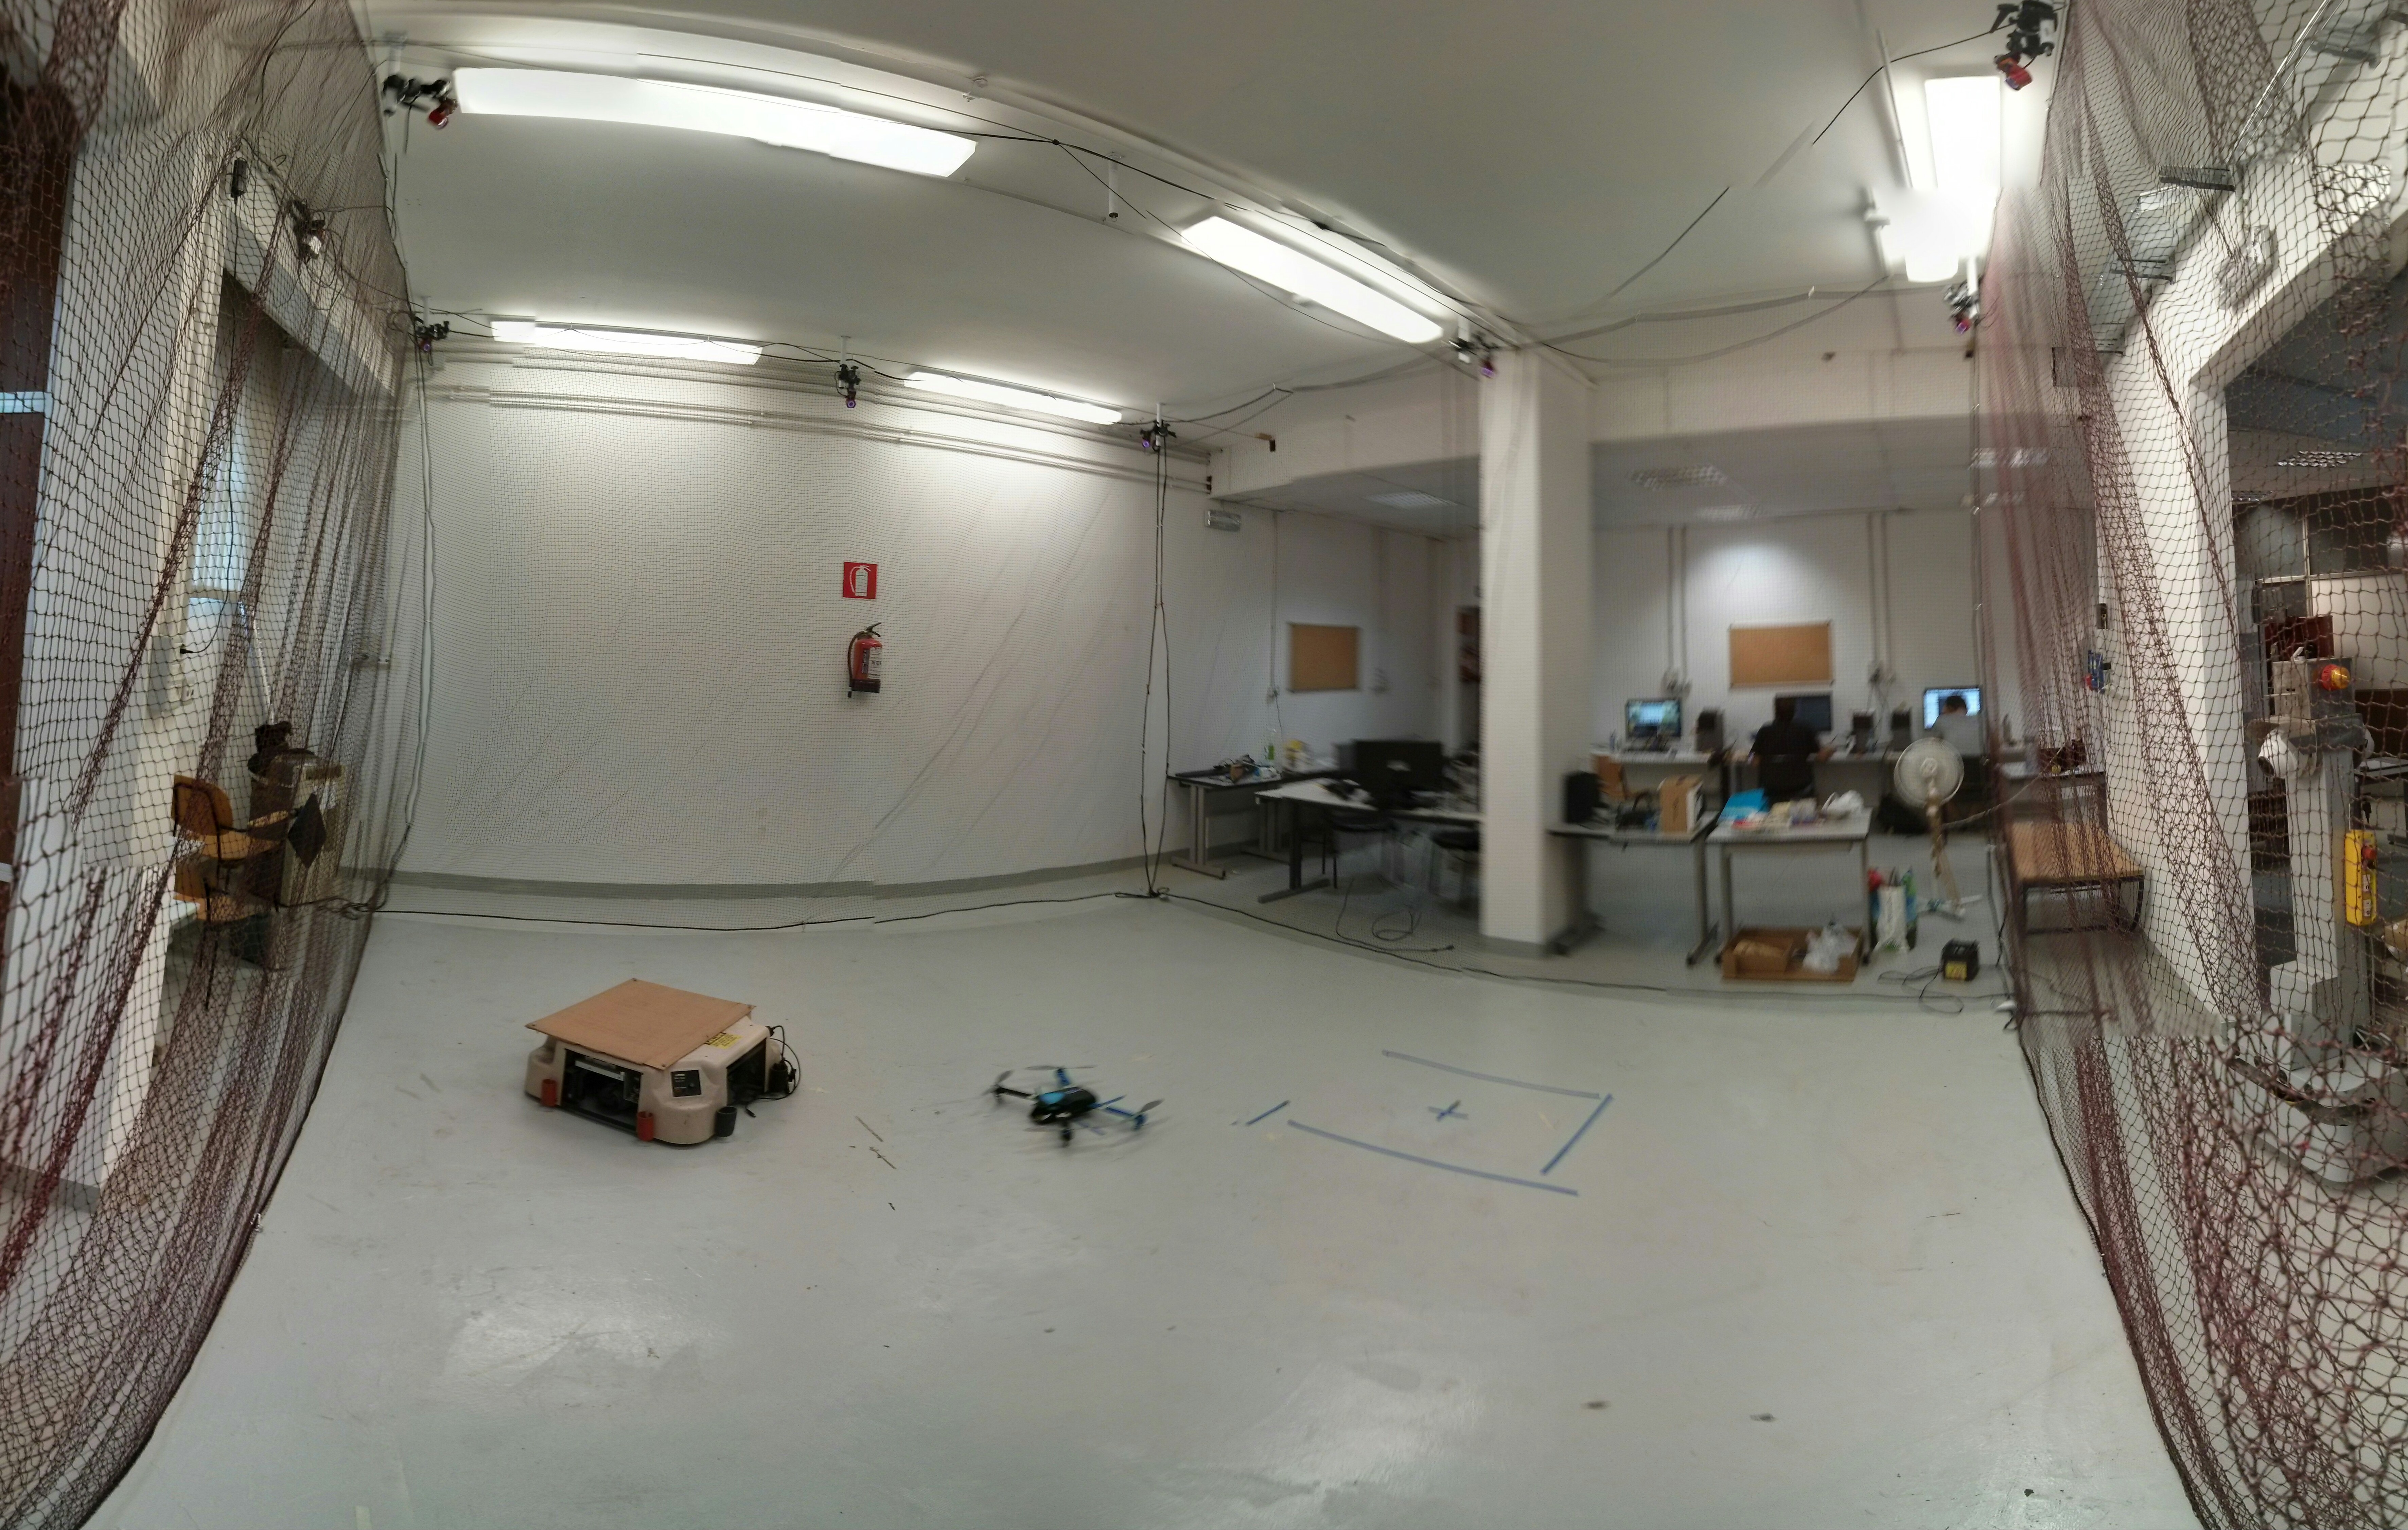
\includegraphics[width=0.8\textwidth]{panoramic.jpg}
 \caption[Flight arena panoramic]{Panoramic view of the flying space.}
 \label{figure:arenapano}
\end{figure}

\begin{figure}[h]
	\centering
	\includegraphics[width=0.6\textwidth]{motiv_panorama.PNG}
	\caption[Flight arena from motive]{Flight arena seen by Motive with a couple of rigid bodies and cameras.}
	\label{figure:arenamotive}
\end{figure}



\section{Overall Integration}
\label{sec:integration}

This section explains to the reader how every part of the setup is interfacing with each other, the flow of data packets from OptiTrack to IRIS and the operation done to the information at each step.

\subsection{Hardware interfaces}

Each camera is equipped with a 5 meters USB cable and, as stated in \ref{sec:mocap}, four cables are connected to one hub and four to the second hub. As outputs, the hubs are equipped with a 5 meter USB cable that can be expanded to 10 meters, those two connection are inputs for the Windows machine. \\*

\noindent
\textbf{Windows machine specs} 
\begin{itemize}

\item OS: Windows 7 
\item Processor: Intel i7 3.60 GHz
\item RAM: 32 Gb
\item Video Card: NVIDIA GTX 970
\item Software tools: Motive

\end{itemize}
This computer is directly connected to a Linux machine through Ethernet cable (RJ-45 connectors). \\

\noindent
\textbf{Linux machine specs} 
\begin{itemize}

\item OS: Ubuntu 14.04 LTS 
\item Processor: Intel i7 2.40 GHz
\item RAM: 8Gb
\item Video Card: NVIDIA GeForce GTX 760M
\item Software tools: Qt C++ Libraries, Px4 build environment \cite{PX4Build}
\end{itemize}
At the end, via USB , a telemetry module (Fig. \ref{figure:telemetry}) is attached to the linux machine.
\begin{figure}[h]
\centering
 \includegraphics[width=0.6\textwidth]{telemetry.jpg}
 \caption[Telemetry module]{Telemetry module from 3d Robotics used to recieve and transmit MAVLink Packages with IRIS.}
 \label{figure:telemetry}
\end{figure}
This radio link allows the control station to communicate with the robot wirelessly with acceptable performance. It is mainly used for acquiring telemetry and robot status, transmit new mission goals, check robot parameters such as controller gains and calibrate onboard sensors. \\*

\noindent
Its main features are \cite{3Dr}:

\begin{itemize}
\item 433 MHz (for Europe).
\item micro usb port: it can be used also from tablets.
\item UART Interface.
\item 2-way full-duplex communication.
\item MAVLink protocol framing.
\end{itemize}
Moreover, IRIS features a standard RC transmitter, shown in figure \ref{figure:iris_planner}, from which the user can operate the robot in three main modes:
\begin{enumerate}
\item Fully manual: radio sticks control directly velocity of the propellers.
\item Semi-auto: height is stabilized, left stick control height position set point while attitude is manual.
\item Fully-auto: horizontal position is stabilized through position feedback, right stick controls x and y set points.
\end{enumerate}

\subsection{Software interfaces}

Motive has the feature to transmit the pose of every tracked rigid bodies through a multicast IP. By this option, the raw pose of the robot is transmitted to the Linux machine. The software architecture running on Linux reads data coming directly from Motive through a \textit{Receiver component}. Without the use of an \textit{adapter component}, since the program is specific for this application, data from Motive is processed as explained in section \ref{sec:adaptframes} at the moment it arrives. In the mean while a position set point is generated inside the architecture, both pose estimation and position set point are packed using MavLink protocol. At the end data is sent through a socket interface an the telemetry module takes care of transmitting everything to IRIS with a rate of approximately 10Hz.

Figure \ref{figure:integration} sums up in a scheme the relation between each part. 

\begin{figure}[h]
\centering
 \includegraphics[width=0.9\textwidth]{integration.png}
 \caption[Setup scheme]{Scheme of the setup with connections between parts}
 \label{figure:integration}
\end{figure}

\subsubsection{Adapting reference frames}
\label{sec:adaptframes}
Motive transmits a 6 degree of freedom pose (position and orientation)respect to a fixed reference frame $\Re^m$ in the form:\\ 
\begin{equation}
Pose^m = \begin{bmatrix}
P^m\\
Q^m
\end{bmatrix}
\end{equation}
 where $P^m\ = \begin{bmatrix}x\\y\\z\end{bmatrix}$ is the position vector and $Q^m =\begin{bmatrix}w\\x\\y\\z\end{bmatrix}$ is the rotation quaternion, everything expressed in Motive reference frame $\Re^m$. \\
 
 \noindent
Now let us define a second reference frame, in this case is a North-East-Down frame \cite{FrameRef}  mainly used in aeronautics and aerial robotics, namely  $\Re^E$. The peculiarity of this reference is that:

\begin{itemize}
\item x axis is aligned with North.
\item y axis is aligned with East.
\item z axis goes down towards the earth.
\end{itemize}

\noindent
The only constraint of $\Re\textsuperscript{m}$ is that y is vertical and x parallel to the ground, hence x and y can be set freely at the moment of cameras calibration Figure \ref{figure:frames} shows both reference.

\begin{figure}[h]
\centering
 \includegraphics[width=0.8\textwidth]{frames.png}
 \caption[NED and Mocap frames]{NED and Mocap frames depicted. X axis in red, y axis in green and z axis in blue}
 \label{figure:frames}
\end{figure}

It is easily shown that the relation between frames is a 90 degree rotation of $\Re\textsuperscript{m}$ over x. Let $R_x(\theta)$ be the rotation matrix on x, $P^b$ arbitrary  3-elements vector column respect to a general base frame $b$, then the following is valid:
\begin{equation}
(P\textsuperscript{m})\textsuperscript{T}R_x(\theta) = P\textsuperscript{E}
\label{eq:adaptframe}
\end{equation}

\begin{equation}
R_x(\theta) = \begin{bmatrix} 1 & 0            & 0 \\
							  0 & \cos(\theta) & -\sin(\theta)\\
                              0 & \sin(\theta) &  \cos(\theta) 
\end{bmatrix}
\label{eq:rotx}
\end{equation}

Putting $\theta = \pi/2$ inside \ref{eq:rotx},then \ref{eq:adaptframe} become:

\begin{equation}
\begin{bmatrix}x&y&z\end{bmatrix}\begin{bmatrix} 1 & 0 & 0 \\
							  					 0 & 0 & -1\\
                              					 0 & 1 & 0
\end{bmatrix} = \begin{bmatrix}x\\z\\-y\end{bmatrix}
\label{eq:rotexplained}
\end{equation}

and

\begin{equation}
P\textsuperscript{E} = \begin{bmatrix}x\\z\\-y\end{bmatrix}
\label{eq:translation}
\end{equation}

where $[x, y, z]$ are the coordinates of $P^m$ in $\Re^m$.\\

\noindent
As regards the rotational part, some comments must be done. Since the applied rotation applied does not influence the estimated attitude, we can safely state that:

\begin{equation}
Q\textsuperscript{E} = \begin{bmatrix}
w\\x\\z\\-y
\end{bmatrix}
\label{eq:quaternion}
\end{equation}
where $[w, x, y, z]$ are the elements of $Q^m$.\\

\noindent
Equations \ref{eq:translation} and \ref{eq:quaternion} describe the relation between $\Re^m$ and  $\Re^E$ in a simple but effective way in fact just by changing the order of the elements of the pose coming out Motive, a pose that IRIS can understand is generated. 
    
% THESIS CHAPTER

\chapter{Modeling IRIS}
\label{chap:fourth
}
\ifpdf
    \graphicspath{{Chapter4/Figures/PNG/}{Chapter4/Figures/PDF/}{Chapter4/Figures/}}
\else
    \graphicspath{{Chapter4/Figures/EPS/}{Chapter4/Figures/}}
\fi

% short summary of the chapter
\section*{Summary}

This part concerns the modeling of the IRIS quad rotor. A model of the quadrotor is necessary to develop a controller and understand better its dynamics. The first part presents some generalities including the reference frames used in order to define the world and the robot. It also contains a list of assumptions done to simplify the model. After this are explained the involved physical principles and the actual derivation of the model.

\section{Generalities}

This section explains general concepts necessary to proceed with modeling. It starts by defining reference frames, then it describes how maneuvering is done and at the end presents general assumptions under which the model is derived.

\subsection{Reference frames}
\label{sec:refframes}
The first element is a world base frame, in Section \ref{sec:adaptframes} is defined $\Re^E$ which is a North East Down frame with its own features. In our case, the world frame is decided freely after calibration. It is the frame respect to which cameras give the pose estimate. Hence $\Re^E$ still keeps its name being world fixed frame but it has no constraint of being oriented North-East-Down. The only constraint for $\Re^E$ is that \textbf{$z$ axis is directed downwards along gravity while $x , y$ axis are parallel to ground.} \\*

\noindent
The next frame is the body frame, namely $\Re^B$. It is attached to the center of mass of the robot with the $x$ axis pointing to the front and $z$ axis downwards, $y$ axis is generated accordingly with the right hand rule (see Figure \ref{figure:refframes}).

 The relation between $\Re^B$ and $\Re^E$ is represented by a transformation matrix, namely ${}^ET_B$ which defines the transformation of $\Re^B$ respect to $\Re^E$ as base frame.

\begin{figure}[h]
\centering
 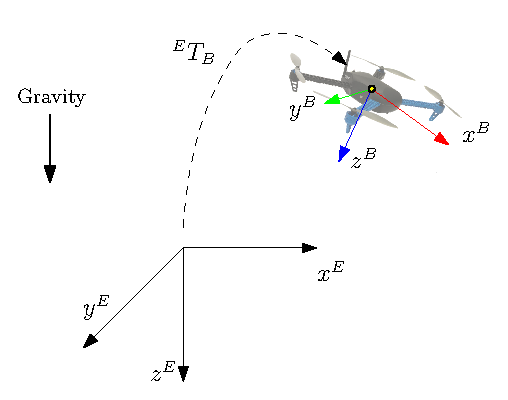
\includegraphics[width=0.8\textwidth]{ref_frames.eps}
 \caption[Reference frames for modeling]{Earth-fixed reference frame,  body-fixed reference frame and the transformation between them.}
 \label{figure:refframes}
\end{figure}

\subsection{General assumptions}

The analysis of this system is pretty complex. In order to simplify the derivation of the model some assumptions are made and some non linearities are disregarded. \\ 

\noindent
When a rotor translates horizontally through the air, the advancing blade has a higher absolute tip velocity and will generate more lift than the retreating blade. The mismatch in lift generates an overall moment on the rotor disk in the direction of the apparent wind causing the blade to flap as shown in figure \ref{figure:refframes} and the generated thrust is inclined respect to the rotor axis. This effect, called \textit{Blade Flapping} is not included in the derived model.

\begin{figure}[h]
\centering
 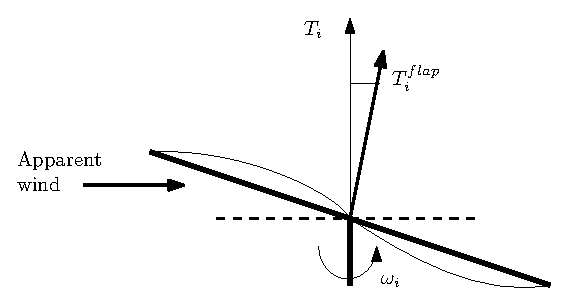
\includegraphics[width=0.7\textwidth]{bladeflap.eps}
 \caption[Blade flapping]{Blade flapping effect. $T_i$ is the ideal vertical thrust while $T_i^{flap}$ is the real thrust vector}
 \label{figure:refframes}
\end{figure}
A second disregarded non linear effect is the \textit{Total Thrust Variation in Translational Flight} \cite{Huang2009}. The analysis of this phenomenon is quite complex and it is described by a  qualitative explanation. When a rotor translates in air, it suffers form apparent wind and an increase of air flux through the blades. This leads to an increase of lift and thrust by the rotor.\par
Moreover, viscous friction experienced by the robot when it moves is negligible at small velocities. The robot can be also considered as a rigid body since there are no significant strains and forces applied which may deform the structure. \\*

\noindent
To summarize, the following assumption are made:
\begin{itemize}
\item Blade Flapping is not considered
\item Thrust Variation in Translational Flight is disregarded
\item Viscous friction (drag) is neglected
\item The robot is considered as a rigid body
\item Motor dynamics are managed internally by the board and not included in the model
\end{itemize}

\section{Transformation matrices}
\label{sec:trasfmatrix}
This Section introduces some mathematical tools necessary to develop a full dynamical model for the quadrotor system. Moreover I will present here the conventions used for representing angles and rotations and the derivation of the matrices involved. \\ 

\noindent
In Section \ref{sec:refframes} I introduced ${}^ET_B$ as the transformation matrix of $\Re^B$ with respect to $\Re^E$. In particular ${}^ET_B$ is a $4\times4$ matrix and has a fixed structure \cite{Khalil2004}: \begin{equation}
{}^ET_B = \begin{bmatrix}
{}^ER_B&&{}^EP_B\\
O_3^T&&1
\end{bmatrix}
\label{eq:transdef}
\end{equation}
in this definition we can see three different terms. ${}^ER_B$ is the rotation matrix of frame $\Re^B$ with respect to $\Re^B$; ${}^EP_B$ = $\begin{bmatrix}x\\y\\z\end{bmatrix}$ is the position of the center of mass of the robot respect to the Earth frame and $O_3$ = $\begin{bmatrix}0\\0\\0\end{bmatrix}$. 

\subsection*{Rotation matrix and angles}

Every rotation in 3D space can be defined by 3 successive rotations about 3 principal axis; we can define separately each rotation matrix about each axis and the multiply them.\\ 

\noindent
Each Right-Hand rotation about a particular axis is defined by a positive angle \cite{Blanco2010} from earth to body frame and the following definitions are true:

\begin{equation}
R_x(\phi) = \begin{bmatrix} 1 & 0            & 0 \\
							  0 & \cos(\theta) & \sin(\theta)\\
                              0 & -\sin(\theta) &  \cos(\theta) 
\end{bmatrix}
\end{equation}

\begin{equation}
R_y(\theta) = \begin{bmatrix} \cos(\theta)  & 0 & \sin(\theta) \\
							  0 & 		      1 &   0\\
                              -\sin(\theta) &  0 &  \cos(\theta) 
\end{bmatrix}
\end{equation}

\begin{equation}
R_z(\psi) = \begin{bmatrix} \cos(\psi)  & -\sin(\psi) &0 \\
							\sin(\psi) & \cos(\psi) &0\\
                              0         & 0          &1 
\end{bmatrix}
\end{equation}
The general rotation matrix can be obtained by multiplying elemantary rotations, but please note that the order is important.\\

\noindent
The most common sequence associated with the name \textit{Euler angles} is $(z, x, z)$ or ${}^ER_B = R_z(\phi)R_x(\theta)R_z(\psi)$.\\ 

\noindent
There is however a more suitable sequence with fits our case. The angles associated with the sequence $(x, y, z)$ are sometimes called \textit{Cardan angles} or \textit{Tait-Bryan angles}. Commonly used in aerospace where $\phi$, $\theta$, and $\psi$ are known respectively as\textbf{ roll}, \textbf{pitch}, and \textbf{yaw}. These angles describe a vehicle whose forward direction is along the positive body-fixed x-axis and the body-fixed z axis downward, like in the case of the quadrotor (see \ref{sec:refframes}). In such configuration, the home position $\begin{bmatrix}\phi\\ \theta \\ \psi \end{bmatrix} = \begin{bmatrix}0\\ 0 \\ 0 \end{bmatrix}$ , is flat and level pointing forward along the world x axis. The non intuitive downward pointing z axis is chosen in order to make a positive change in $\theta$ correspond to pitching upward \cite{Diebel2006}. \\

\noindent
Having said that, the multiplication order used is $(x , y , z)$. Developing the calculations, the general rotation matrix becomes:\begin{equation}
{}^ER_B = R_x(\phi)R_y(\theta)R_z(\psi) = \begin{bmatrix} 
c_\theta c_\psi && s_\phi s_\theta c_\psi - c_\phi s _\psi &&  c_\phi s_\theta c_\psi + s_\phi c _\psi \\
c_\theta s_\psi&& s_\phi s_\theta s_\psi + c_\phi c _\psi && c_\phi s_\theta  s_\psi - s_\phi c _\psi \\
-s_\theta && c_\theta s_\phi  &&  c_\theta c_\phi 
\end{bmatrix}
\label{eq:rotmatrix}
\end{equation}where $c = cos$ and $s = sin$ for simplicity, Moreover, the following limits are true by definition: \begin{itemize}
\item $ -\pi < \phi < \pi$
\item $ -\pi/2 < \theta < \pi/2$
\item $ -\pi < \psi < \pi$
\end{itemize}
while the following shows the transformation from the derivative of the Euler angles to the angular velocity in the body frame\cite{Friis2009}:
\begin{equation}
W = \begin{bmatrix} 
1 && 0 && -s_\theta\\
0 && c_\phi && c_\theta s_\phi \\
0 && -s_\phi && c_\theta c_\phi
\end{bmatrix}
\end{equation}
Please also note that ${}^ER_B$ is an orthonormal 3x3 matrix so its inverse it is equal to its transpose \cite{Khalil2004}, hence $({}^ER_B)^{-1} = ({}^ER_B)^{T}$ = ${}^BR_E$.

\section{Propulsion and controls}
\label{sec:propulsion}

The four motors installed are responsible of the propulsion of the quadcopter. Each rotor-motor couple rotates with an angular velocity $\omega_i$ and generates: an upward lifting force $f_i$ parallel to the body z axis $z^B$ and a reaction torque $\tau_r$. This quantities approximated by a linear model where: \begin{equation}
f_i = k \omega_i ^ 2
\label{eq:fi}
\end{equation}
\begin{equation}
\tau_i = k_d \omega_i ^ 2
\label{eq:taui}
\end{equation}
$k$ and $k_d$ are positive constants depending on atmospheric conditions and blade geometry. This constants can be identified through dynamical tests but in this case they are provided in the autopilot configuration file.\\

\begin{figure}[h]
\centering
 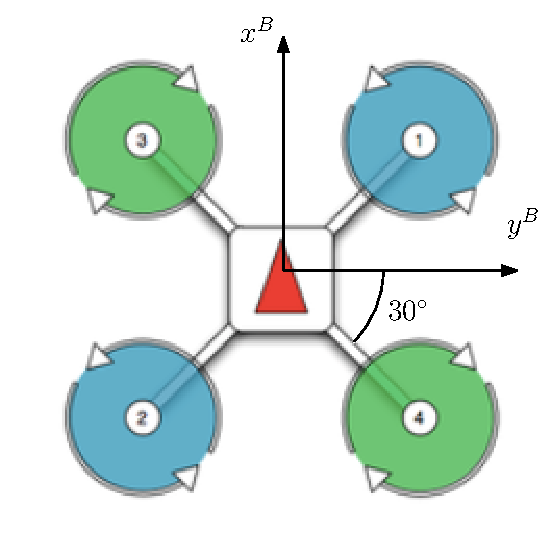
\includegraphics[width=0.5\textwidth]{top_iris.eps}
 \caption[Motor rotations]{Motor labeling and spinning}
 \label{figure:motorspin}
\end{figure}

\noindent
The total thrust $T$ acting on the robot's center of mass, parallel to $z^B$ and directed upwards is:
\begin{equation}
\boldsymbol{T^B}=\begin{bmatrix}0\\0\\\sum_{i=1}^{4}f_i
\end{bmatrix}
\label{eq:T}
\end{equation}
while the total moments
\begin{equation}
\tau_\phi = \sum_{i=1}^{4}d_1\sin(\alpha_i) f_i
\label{eq:tauph}
\end{equation}
\begin{equation}
\tau_\theta = -\sum_{i=1}^{4}d_i\cos(\alpha_i) f_i
\label{eq:tauth}
\end{equation}
\begin{equation}
\tau_\psi = \sum_{i=1}^{4}\sigma_i\cos(\alpha_i) \tau_i
\label{eq:taups}
\end{equation}
where $f_i$ and k are defined in \eqref{eq:fi}; $\tau_i$ and $k_d$ in \eqref{eq:taui}; $d_i$ is the distance from the center of the rotor to the center of mass; $\sigma_i$ is positive if $\omega_i$ is positive and negative otherwise; $\alpha_i$ is the angle between the vector going from the center of mass to the \textit{i-th} motor and $y^B$ ($30^\circ$ for IRIS).\\

\noindent
By rearranging \eqref{eq:tauph}, \eqref{eq:tauth} and \eqref{eq:taups} in matrix form:
\begin{equation}
\begin{bmatrix}
T^B\\\tau_\phi\\\tau_\theta\\\tau_\psi
\end{bmatrix} = \begin{bmatrix}
k&&k&&k&&k\\
k d_i \sin(30)&&-k d_i \sin(30)k&& -d_i \sin(30)&&d_i \sin(30)\\
-k d_i \cos(30)&&-k d_i \cos(30)k&& d_i \cos(30)&&d_i \cos(30)\\
k_d&&-k_d&&-k_d&&k_d
\end{bmatrix} \begin{bmatrix}
\omega_1^2\\\omega_2^2\\\omega_3^2\\\omega_4^2
\end{bmatrix}
\label{eq:inputmix}
\end{equation}

\begin{equation}
\begin{bmatrix}
T^B\\\tau_\phi\\\tau_\theta\\\tau_\psi
\end{bmatrix} = H \begin{bmatrix}
\omega_1^2\\\omega_2^2\\\omega_3^2\\\omega_4^2
\end{bmatrix}
\label{eq:inputmixmatrix}
\end{equation}
where in this case $T^B$ is the value of the force directed through $z^B$, $\tau_\phi$ is the torque along $x^B$, $\tau_\theta$ is the torque along $y^B$ and finally  $\tau_\psi$ is the torque along $z^B$. The force $T^B$ is responsible of the translation or the body frame while the three torques generate rotations in each principal axis.

Figure \ref{figure:motorspin} shows how motors are labeled in IRIS and the respective direction of rotation while \ref{figure:forces} is a diagram with the applied forces on the rigid body.

\begin{figure}[h]
\centering
 \includegraphics[width=0.7\textwidth]{forces.png}
 \caption[Quad dynamics]{Dynamics of the copter. Assume that x axis points towards the red propeller for simplicity, black arrows are the generated forces $f_i$ from aerodynamics. Green arrows represent forces and torques generated combining the rotational speed of the propellers.}
 \label{figure:forces}
\end{figure}


\section{Complete model}

Equation \eqref{eq:inputmix} shows the relation between the squared velocity of each rotor and the generated force and torques  . Hence the problem can be split in two parts, aerodynamics and equations of motion. Therefore, \textbf{the model is defined as a rigid body on which one external force $T^B$ and three external torques $[\tau_\phi ; \tau_\theta ; \tau_\psi]$ are applied.} Those external perturbations are calculated in \ref{sec:propulsion} and they correspond to the aerodynamic propulsion of the blades. 

\subsection{Rigid body equations}

In order to develop the full dynamical model, the control signals must be introduced. Let us define $U$ as a 4-element control vector, then the following is true by definition:
\begin{equation}
\textbf{U} = \begin{bmatrix}
T^B\\\tau_\phi \\ \tau_\theta \\ \tau_\psi
\end{bmatrix}
\label{eq:inputs}
\end{equation}
Let us also approximate the inertia of the blades equal to zero for simplicity as in \cite{Vendittelli}. We can define the following quantities:\begin{itemize}
\item $\boldsymbol{r}$ = $\begin{bmatrix} x\\y\\z\end{bmatrix}$ position of the robot in Earth frame.
\item $\boldsymbol{\eta}$ = $\begin{bmatrix} \phi\\\theta\\\psi\end{bmatrix}$ attitude of the quadcopter respect to earth frame (roll, pitch, yaw) presented in \ref{sec:trasfmatrix}.
\item $\boldsymbol{\Omega}$ = $\begin{bmatrix} p\\q\\r\end{bmatrix}$ body angular speed respect to each axis in body frame.
\item ${}^ER_B = R(\eta)$ rotation matrix encoding body attitude defined in \ref{sec:trasfmatrix} such that $\boldsymbol{x^E} =  R(\eta) \boldsymbol{x^B}$.

\item $W = W(\eta)$ Euler angle rate matrix defined in \ref{sec:trasfmatrix} relating $\boldsymbol{\Omega}$ with $\dot{\boldsymbol{\eta}}$ 
\end{itemize}
The dynamics of the quadcopter can be described by the use of Newton-Euler cardinal equation for motion of a general 6 DOF rigid body suffering from an external force and torque. The four equations for the undergoing motion are defined as the following:

\begin{align}
\label{eq:rigidb1}
\boldsymbol{\dot{r}}& = \boldsymbol{v}\\ \label{eq:rigidb2}
m\boldsymbol{\dot{v}}& = \boldsymbol{F}\\ 
\label{eq:rigidb3}
\dot{R}& = R\Omega_\times\\ 
\label{eq:rigidb4}
I\boldsymbol{\dot{\Omega}}& = -\boldsymbol{\Omega} \times I\boldsymbol{\Omega} + \boldsymbol{\tau}
\end{align}
\noindent
where the vector $\boldsymbol{F}$ is the resultant of all the external forces applied on the rigid body's center of mass and $\boldsymbol{\tau}$ is the total torque acting on the body. $\Omega_\times$ is a $3\times3$ skew symmetric matrix such that $\Omega_\times \boldsymbol{v} = \boldsymbol{\Omega} \times \boldsymbol{v}$ for the vector cross product $\times$ and any vector $\boldsymbol{v}$ \cite{Mahony2012}. The inertia matrix is diagonal of the form
\begin{equation}
	I=\begin{bmatrix}
	I_{xx}&&0&&0\\0&&I_{yy}&&0\\0&&0&&I_{zz}
	\end{bmatrix}
\end{equation}
due to the symmetries of the body about principal axis while $m$ is the total mass of the robot.

\paragraph{Equations for translation}

Since viscosity in air is not considered, the total forces acting on the robot are the gravity $m\boldsymbol{g}$ and the thrust generated by the rotors $\boldsymbol{T^B}$ calculated in equation \eqref{eq:T}. \\

\noindent
Let us define $U_1 = T^B$ meaning the first element of the control vector $U$ introduced in \ref{eq:inputs} where $T^B$ is the module of the thrust directed along $z^B$ (see equation \ref{eq:inputmix}).
As consequence \eqref{eq:rigidb2} can be written as follows:
\vspace{1ex}
\begin{equation}
\vspace{1ex}
\boldsymbol{\dot{v}} = \frac{1}{m}\left(\begin{bmatrix}0\\0\\mg\end{bmatrix}^E + R\begin{bmatrix}0\\0\\U_1\end{bmatrix}^B\right)
\label{eq:rigidb2new}
\end{equation}
\textbf{Note:} the first column vector in equation \eqref{eq:rigidb2new} is the gravity force and is directed along $z^E$ on its positive direction (downwards). The second column vector is the thrust in body frame which is along $z^B$ pointing to its positive direction. The multiplication with the rotation matrix $R$ rotates the thrust vector expressing in in earth frame since $\boldsymbol{v}$ must be expressed in earth frame.\\

\noindent
\paragraph{Equations for rotation}
The total torques acting on the robot are those originated by the commanding maneuvers calculated in equation \ref{eq:inputmix} and the gyroscopical effect induced by the rotating blades. \par The gyroscopic torques can me neglected because the mass of the blades is very low, then the total torque applied on the rigid body is the one originated by the lifting forces and we have that $\boldsymbol{\tau} = \begin{bmatrix}
\tau_\phi\\\tau_\theta\\\tau_\psi
\end{bmatrix}$. Those values are namely the second, the third and the forth elements of the control vector $U$ hence equation \ref{eq:rigidb4} becomes:
\vspace{1ex}
\begin{equation}
\vspace{1ex}
\boldsymbol{\dot{\Omega}} =I^{-1}\left(\begin{bmatrix}
U_2\\U_2\\U_4
\end{bmatrix} -\boldsymbol{\Omega} \times I\boldsymbol{\Omega}\right)
\label{eq:rigidb4new}
\end{equation}
where it assumes this simple form due to the assumption of null gyroscopic effects.\\

\noindent
Moreover, equation \eqref{eq:rigidb3} can be substituted by the explicit relation between angle rates in earth and in body frame through the matrix $W$ \cite{Kendoul2007}. Thus, equation \eqref{eq:rigidb3} is replaced by:
\vspace{1ex}
\begin{equation}
\vspace{1ex}
\boldsymbol{\dot{\eta}} = W\boldsymbol{\Omega}
\label{eq:rigidb3new}
\end{equation}
where, for recalling, $\boldsymbol{\Omega}$ is the angular velocity vector in body frame.

\subsection*{Full non linear model}
Expanding equations \eqref{eq:rigidb1}, \eqref{eq:rigidb2new}, \ref{eq:rigidb3new} and \eqref{eq:rigidb4new} we obtain the full mathematical model represented by the following differential equations:
\vspace{2ex}
\begin{equation}
\vspace{2ex}
\left\lbrace
	\begin{aligned}
		\dot{x}& = v_x \\
		\dot{y}& = v_y \\
		\dot{z}& = v_z \\
		\dot{v_x}& = -\frac{U_1}{m}(\cos(\phi)\sin(\theta)\cos(\psi) + \sin(\phi)\sin(\psi) \\
		\dot{v_y}& = -\frac{U_1}{m}(\cos(\phi)\sin(\theta)\sin(\psi) + \sin(\phi)\cos(\psi) \\
		\dot{v_z}& = g - \frac{U_1}{m}(\cos(\phi)\cos(\theta) \\
        \dot{\phi}& = p - r \sin(\theta) \\
        \dot{\theta}& = q \cos(\phi) + r\cos(\theta) \sin(\phi) \\
        \dot{\psi}& = r \cos(\phi) \cos(theta) - q \sin(\phi)\\
        \dot{p}& =\frac{1}{I_{xx}}(U_2 + qr(I_{yy} - I_{zz})) \\
        \dot{q}& =\frac{1}{I_{yy}}(U_3 + pr(I_{zz} - I_{xx})) \\
        \dot{r}& =\frac{1}{I_{zz}}(U_4 + pq(I_{xx} - I_{yy})) \\
     \end{aligned}
     \right.
\label{eq:mathfullmodel}
\end{equation}
I want to stress that this model does not take into account factors such as aerodynamic drag, ground effect, blade-flapping, gyroscopic effects or advanced aerodynamics phenomenons. Even with this approximations, this model is the most used in the research because it assures good precision.

\subsubsection*{Simplified model}
Further simplifications can be applied, let us consider the quadrotor in the flat position and now assume that the variation of roll and pitch angles are reasonably small. This is a logical assumption since the quadcopter is designed to fly around such configuration; we can assume that $\phi \approx 0$ and $\theta \approx 0$ and the matrix $W$ becomes an identity matrix as consequence. Therefore under those conditions we have that $\boldsymbol{\dot{\eta}} = \boldsymbol{\Omega}$ and the model is:

\vspace{2ex}
\begin{equation}
\vspace{2ex}
\left\lbrace
	\begin{aligned}
		\dot{x}& = v_x \\
		\dot{y}& = v_y \\
		\dot{z}& = v_z \\
		\dot{v_x}& = -\frac{U_1}{m}(\cos(\phi)\sin(\theta)\cos(\psi) + \sin(\phi)\sin(\psi) \\
		\dot{v_y}& = -\frac{U_1}{m}(\cos(\phi)\sin(\theta)\sin(\psi) + \sin(\phi)\cos(\psi) \\
		\dot{v_z}& = g - \frac{U_1}{m}(\cos(\phi)\cos(\theta) \\
        \dot{\phi}& = p \\
        \dot{\theta}& = q  \\
        \dot{\psi}& = r \\
        \dot{p}& =\frac{U_2}{I_{xx}} \\
        \dot{q}& =\frac{U_3}{I_{yy}} \\
        \dot{r}& =\frac{U_4}{I_{zz}} \\
     \end{aligned}
     \right.
\label{eq:mathlinlmodel}
\end{equation}

\noindent
Please note that only the rotational dynamics are simplified. This model, even with the various assumptions and the linearization, is often used to try simple control algorithm and design linear controllers. In our case it is useful since this project do not include the study on aggressive maneuvering or high velocity motions, the small angle variation for roll and pitch is a valid assumption in fact thi model is used to design controllers for hovering. 

\begin{table}[h]
\centering
\begin{tabular}{c c r}
\hline
$m$ & total mass of the robot & $1.308$ Kg \\
$I_xx$& inertia for the x axis& $0.0018$ Kg $m^2$ \\
$I_yy$& inertia for the y axis& $0.0012$ Kg $m^2$ \\
$I_zz$& inertia for the z axis& $0.0027$ Kg $m^2$ \\ \hline
$k$   & thrust coefficient & $0.1$ \\
$k_d$ & drag coefficient & $ 0.1$ \\
\end{tabular}
\caption{IRIS parameters. The moment of inertia are taken from the autopilot parameters file while the aerodynamic coefficients are taken from the blade technical sheet.}
\end{table}
















% THESIS CHAPTER

\chapter{Control and state estimation}
\label{chap:fifth
}
\ifpdf
    \graphicspath{{Chapter5/Figures/PNG/}{Chapter5/Figures/PDF/}{Chapter5/Figures/}}
\else
    \graphicspath{{Chapter5/Figures/EPS/}{Chapter5/Figures/}}
\fi

% short summary of the chapter
\section*{Summary}
Due to the nature of the dynamics of the quadrotor, several control algorithms have been applied to it. As to be expected, each control scheme has its advantages and disadvantages. This chapter presents the techniques that are used to estimate the system's states and to stabilize IRIS which are currently implemented in the PX4 Firmware.\par After a quick overview of the estimator modules, the controller architecture is presented. Moreover, this chapter explains in details how the on board autopilot interfaces with the software architecture and which modules are involved.

\section{Introduction to the PX4 Flight Stack}

The PX4 Flight Stack denotes the list of all the applications running on board the PixHawk. Those modules provide the services and methods which are necessary to manage the radio communications, inter process message pass-through, data logging, state estimation, control, high level states and low level communication with motors and sensors.

\subsection{Message pass-through}
The core on board applications are started at system startup, others can be started via the NuttShell or forced to startup by inserting them in the start boot file. Every application runs independently with its own frequency; the interfaces between processes are managed by \textit{uOrb} middleware (Micro Orb) which, with the use of topics, guarantees the message pass-through for data packets over named buses. Those topics encode structs and they are pre defined. In PX4, a topic (often called node) contains only one message type, e.g. the \textit{vehicle attitude} topic transports a message containing the attitude struct (roll, pitch and yaw estimates).\par Nodes can publish a message on a bus/topic or subscribe to a bus/topic. They are not aware of who they are communicating with. There can be multiple publishers and multiple subscribers to a topic. This design pattern prevents locking issues and is very common in robotics. \textbf{To make this efficient, there is always only one message on the bus and no queue is kept}. The total list of \textit{uOrb} topics can be found in the uOrb folder of the PX4 Firmware since the online documentation is not updated. \\

\noindent
The external communication (through radio link) is managed by mavlink, previously presented in section \ref{sec:mavlink}, however Mav packets are translated in uOrb topics internally.   
        
% THESIS CHAPTER

\chapter{Software architecture}
\label{chap:sixth
}
\ifpdf
    \graphicspath{{Chapter6/Figures/PNG/}{Chapter6/Figures/PDF/}{Chapter6/Figures/}}
\else
    \graphicspath{{Chapter6/Figures/EPS/}{Chapter6/Figures/}}
\fi

% short summary of the chapter
\section*{Summary}

This chapter introduces the reader to the software architecture running off board on Linux. The introduction presents a  general overview on software architectures, expressed the needs of such a system and in particular it describes the environment and software tools involved. Next section presents the design pattern according to which the sofware is organized explaining its advantages and limitations. Then the software components are described with more detail one by one and the results of the experiments are reported. 
\section{Introduction to the proposed architecture}

Architecture is usually intended as the process or product of planning, designing and constructing entities. Usually those entities refer to buildings and structure but the concept can be extended to vehicles, electrical and electronics components or softwares. The architect decides where to locate different elements such as walls, doors columns and windows and connect them in harmony with structural consistency. In the same way the software engineer connect, design and locate different software components. A component could be a program implementing an algorithm, some conversion or a graphical user interface. The basic idea of architecture definition is to design software structure and object interaction before the detailed design phase. Although serious architecture definition is being suggested for large projects only, arguably any software construction or implementation work must be preceded by an architectural design \cite{msdn}.
 \subsection{Motivations}
At this point one may ask: why do we need to define an architecture? The answer is pretty simple: it makes things easier,more clear and simpler. A software architecture is an abstract view of a software system distinct from the details of implementation, algorithms, and data representation. Thus it gives an organizational map we may follow during the design flow. A well written software architecture should:
 \begin{itemize}
 \item Provide flexibility and adaptability.
 \item Allow for interoperability with other softwares and elements in general.
 \item Provide control on the system.
 \item Reduce maintenance time and cost.
 \item Help developers improving the software.
 \end{itemize}
Reusability is a key aspect in design of this kind of systems. One software may be used for a different application changing only few parameters or modules. Each module should be self contained and work as a \textit{black box}, meaning that once the input and output are defined, the actual implementation has no importance. Standardization clearly takes an important role, the way components communicate for example must be known by the developer. If different modules speak the same \textit{language} or \textbf{protocol} (e.g. the MavLink standard) in engineering terms, it is simpler to interface them. Moreover, a self contained module is more easy to maintain and expand because developers can focus on that specific aspect without knowing what is happening outside. In that way specialist in different fields can cooperate designing each own part. The role of the software engineer is on one hand to design software components, and on the other to integrate them with modules written by others. Finally, it seems trivial to point it out, but the architecture must work respecting the specifications and providing the needed control on the system. 

\paragraph{Note:}This software was designed ad-hoc for indoor flight because there were not any other alternatives. Every control station is specialized for outdoor flight which is not our case. Moreover this software aims to become a research platform for controlled environments (e.g. indoor flight) for anyone who wants to contribute.
\subsection{Programming environment and tools}

Every job has its own tools. In order to implement what we theorized in the introduction of this chapter we need to rely on software tools. There are many different frameworks which helps developers in implementing their own ideas.

 The state of the art and widely used framework in robotics is ROS or Robotic Operative System \cite{ROS}. ROS is a publish/subscrbe middleware meaning that it packs function classes and features which provide inter process communication. It supports most of the libraries used in robotics for path planning, computer vision, control and so on. The main feature is that ROS is very easy to use and let the user create different parallel processes (or nodes) without focusing on low level aspects. As consequence of that, the designer can concentrate on the actual problem he is working on and leave lower level managing such as shared variables, timing or buffers to ROS. This feature increase exponentially the productivity while writing a program. Moreover, ROS is becoming a standard in research and also industry. That means that many packages are available online that one can use, the community and the documentation are superb and it is open source. This framework has all the features needed for a good base of a software architecture.
 
 However there are three main reason which made me discard ROS as a choice. First of all, as stated in chapter \ref{chap:second}, most of the control stations are written with Qt libraries. Since one may thing to include this architecture in one of them in the future, could be an idea to go in the same direction. The second one is that the very first module of this architecture was written by a PhD student, Tommaso Falchi Delitalia, using the Qt framework. It was nice to have a base starting point and expand from that. The last reason, but not the least, is that ROS gave me important delay problems when I tried to integrate mavlink in it. Mavlink is not fully supported but some packages, in development, are out there and they simplify the design such as the acquisition of data from Motive \cite{optiros}.

Hence the used tools are \textbf{Qt libraries} \cite{qt} while the chosen programming language is C++, widely used and a standard in robotics. Qt is a powerful framework that let the user create user interfaces with good performance. It packs a set of classes, functions and libraries for almost any kind of needs. Moreover is portable on different platforms such as tablets, smartphones and the most important operative systems. for this reason it is used to implement control station, applications like navigators and vehicles control panels.

The functions and classes used for this project are debugging functions to print logs, multi-threading classes to implement parallel modules, sockets interfaces classes and system functions to manage lower level services.By far Qt seems perfect, it provides a very easy access to many features, the documentation is very clear and the learning time is pretty low. The very big disadvantage is the lacking of inter process communication support. The pub/sub design is perfect for robotics application but Qt does not provide any help on that, at least for now. Thus the drawbacks of using this kind of framework is that we need to manage inter process message pass-through in some way. This is done and explained in section \ref{sec:sofdescrip}. A porting on ROS could be interesting in the future, after solving delay related issues, for research interests.
\section{Design patterns}
\label{sec:patterns}
In the course of history the concept of \textit{style} was born and developed. An architectural style is characterized by the features that make a building or other structure notable and historically identifiable. The style identifies a common trend, elements or rules that are used in a particular period or by a group of people during the design flow. The same concept evolved to various disciplines; in computer science, the architecture "style" is often called \textbf{Design Pattern}. The analogy with building design is strong, the formal definition of design pattern is the following: 
\paragraph{Definition of Design Pattern}:  \textit{a design pattern is a general reusable solution to a commonly occurring problem within a given context in software design.} \\

\noindent
The pattern is a description or template for how to solve a problem that can be used in many different situations, usually for groups of problems. Similarly to the architecural style, the software pattern is defined by common structures, participants, communications, protocols and standards. Design patterns can speed up the development process by providing tested, proven paradigms. Thus the software architecture is defined by its style, namely design pattern, which is chosen among the available ones. First step to follow during the prototyping of the software is to have clear in mind which kind of problem we are facing and which are the constraints of the system. 

At this point the reader should ask how is the software interfacing with the robot and which kind of control does it have on the system. As stated in chapter \ref{chap:fifth}, the external signals that are input of the on board flight stack are the 4-D position value from the mocap and the 4-D position set point. By 4-D we mean a vector composed with [x, y, z, yaw] since roll and pith are estimated on board (see figure \ref{figure:controlarch}). Moreover the following goal is set:
\paragraph{Goal:} \textit{The robot must be able to perform some kind of tasks provided by the user and in the most autonomous way possible.} \\

\noindent
In other words, the user provides a list of tasks he wants to perform with the robot and the software architecture guide the system by sending mocap values and position set points. The first scheme of the software is represented in figure \ref{figure:inout}. 
\begin{figure}[h]
\centering
 \includegraphics[width=0.8\textwidth]{first_arch.png}
 \caption[In-out relation]{Input / Output relation of the software architecture.}
 \label{figure:inout}
\end{figure}
The scheme explains the input output relation, where as input there is a C-struct describing the task and as output MavLink messages for mocap estimate and position set point. Nevertheless, the real structure is a bit different. I decided to put the task list inside the software architecture as a nested component. The main reason for that is simplicity, in the future one may encode the list in a text file as input of the software. See figure \ref{figure:inoutnest} for the actual implementation.

\begin{figure}[h]
\centering
 \includegraphics[width=0.8\textwidth]{nested_arch.png}
 \caption[In-out relation for the nested arch]{Input / Output relation of the software architecture with nested component.}
 \label{figure:inoutnest}
\end{figure}

\subsection{Behavioral architecture}
At this point, a way to model the problem is necessary. Let us start from the goal: there a list of tasks and the robot must executes them sequentially and autonomously. Thus, the concept of task arises. The task is defined as \textit{a definite piece of work assigned to the robot and performed by acting on the environment}. 

\paragraph{Defined tasks} Which kind of tasks may be performed by IRIS? The first step is to define the essential tasks of navigation which are:
\begin{itemize}
\item Take off - from the ground or an horizontal plane.
\item Land - land on actual position.
\item Move - go to a target point in 3-D space.
\item Rotate - Change yaw value to a desired one.
\end{itemize}
Moreover a fifth task is added but discussed in \ref{chap:seventh} which is land on a mobile platform. \newline \\
In order to make things more flexible, each task has a set of parameters used to influence the performance during the execution and to adapt to the environment. A detailed explanation is given in \ref{sec:auto}. Furthermore, it is evident that most of the tasks described involve in some way a location in space. Hence the task is modeled in a C-struct with two elements: position and action. In the software the task takes the name \textbf{node} which is often used in control stations and graph based application.

 Table \ref{tab:node} describes the node struct. The position \textit{p} is itself a struct with four elements (x,y,z,yaw) encoding the 4-D pose in space. The action \textit{a} is another stuct with a char value to identify the type of action and a parameter array which can be filled with values. The meaning of the parameter array changes depending on the action.
\begin{table}[h]
\centering
\begin{tabular}{llll}
\multicolumn{4}{c}{\textbf{Node} struct} \\
\hline
position \textit{p} &     &       &           \\
           & \textit{x}   & double & meters    \\
           & \textit{y}   & double & meters    \\
           & \textit{z}   & double & meters    \\
           & \textit{yaw} & double & radiants  \\ \hline
action \textit{a}   &     &       &           \\
           & \textit{id}  & char  &           \\
           & \textit{params}    &  double[4]     & \\
\end{tabular}
\label{tab:node}
\caption{Node struct descripton}
\end{table}
Those elements are necessary in order to choose which design pattern is suitable in this environment.
\newline \\
\noindent
Taking inspiration from biology and observing how simple animals interacts with the environment, robotic schemes and models may be derived. Biologist discovered that animals like frogs, pigeons insects and fishes exhibit different behaviors depending on the sensory inputs they receive from the environment. With this simple method they are able to survive, hunt and navigate. Two different examples explain the concept very well.

Frogs eyes are able to detect movement. In particular on layer detects small moving objects like flies and another layers detects big object, for example predators. The two layers work in parallel. When the first one is activated, meaning that there is food in the proximity, the frogs jumps towards the pray. On the other hand, when the second layer is triggered 






\section{Software description}
\label{sec:sofdescrip}

\subsection{General scheme}
\subsection{Service modules}
\subsubsection{NatNet Reciever}
\subsubsection{Position Dispatcher}
\subsection{Manual Control}
\subsection{Automatic Control}
\label{sec:auto}
\subsection {Executioner}

\section{Experiments and results}
% THESIS CHAPTER

\chapter{Landing on a mobile platform}
\label{chap:seventh
}
\ifpdf
    \graphicspath{{Chapter7/Figures/PNG/}{Chapter7/Figures/PDF/}{Chapter7/Figures/}}
\else
    \graphicspath{{Chapter7/Figures/EPS/}{Chapter7/Figures/}}
\fi

% short summary of the chapter
\section*{Summary}
% THESIS CHAPTER

\chapter{Results}
\label{chap:fifth
}
\ifpdf
    \graphicspath{{Chapter8/Figures/PNG/}{Chapter8/Figures/PDF/}{Chapter8/Figures/}}
\else
    \graphicspath{{Chapter6/Figures/EPS/}{Chapter8/Figures/}}
\fi

% short summary of the chapter
\section*{Summary} 
%%%%%%%%%%%%%%%%%%%%%%%%%%%%%%%%%%%%%%%%%%%%%%%%%%%%%%%%%%%%%%%%%%%%%%%%%%%%%%%%
%2345678901234567890123456789012345678901234567890123456789012345678901234567890
%        1         2         3         4         5         6         7         8
% THESIS CONCLUSIONS
\def\baselinestretch{1}
\chapter{Conclusions}
\label{chap:conclusions}
\ifpdf
    \graphicspath{{Conclusions/Figures/PNG/}{Conclusions/Figures/PDF/}{Conclusions/Figures/}}
\else
    \graphicspath{{Conclusions/Figures/EPS/}{Conclusions/Figures/}}
\fi
\def\baselinestretch{1.66}

This project resulted in a complete integration between different heterogeneous modules. The goal is to stabilize and perform a number of tasks with an IRIS quadcopter with the help of position feedback given by a motion capture system. The course of this project is identified by important steps, or milestones at this point, which reflect the followed plan and highlight important informations that the reader should understand. \\

\noindent
A crucial phase is the integration between different systems which is a necessary condition in order to perform any kind of research. This aspect is treated in this thesis since it is the fist time that an experimental setup, intended for the investigation of aerial vehicle technology, was used in the University of Genoa. In particular, by tweaking internal and external parameters, the system is able to localize himself in a controlled environment without the use of the GPS. Key point of this phase is the adaptation of the two coordinate system: mocap and earth frame. I would like to stress that the integration phase lead to the discovery of a number of bugs which, after being corrected, were pushed to the original PX4 repository and accepted by the administrators. This made me a contributor of the project PX4/PixHawk and permitted some PX4 users to continue their work. The integration of the on board estimator with a position feedback signal is the final step of this first phase. With the trick of faking the earth magnetic field, the system is free from any external source other than the mocap and we can place earth frame wherever is convenient.

I was involved in the relocation of the equipment in the new laboratory, thus a physical integration was also performed solving a number of logistic issues  Thanks to the setup of this new environment, a new study platform is available from now on giving the possibility to expand the research field.

A second milestone is the stabilization of the quadrotor on a position set point. This phase was possible only after modifying the structure of the on board position controller, since it was designed only to fly with GPS, and after tuning controller parameters specifically for IRIS. \\

\noindent
Nevertheless, the most important landmark is the design, development and testing of the software architecture. A simple behavioral system takes place of the so called ground station. This software is intended for indoor flight and specifically designed for this application; however it can potentially drive any setup with an OptiTrack based motion capture and a MAVLink based quadrotor. Moreover, after a number of investigations, I can safely state that there are not other choices which replace a normal ground station for controlled environments. The aim of this platform is to become, or at least try, an open project in which users and developer can add their own ideas. The system is able to manage complex task lists provided by the user and execute them sequentially in an autonomous way. Autonomy in fact is one of pillars over which the architecture lays its foundations but it shares the weight of the structure with a second one: expandability and modularity. Since each behavior is independent from the others, the system is very modular and consequently expandable. \\

\noindent
Last but not the least, an important phase is the design of an algorithm for landing on a mobile platform using position control and no velocity knowledge of the target. A simple but very effective PI plus offset law is derived and used. Surprisingly we proved to be very effective and, combined with a linear descent relation depending on horizontal error, we achieved the goal. The importance of this outcome relies not only on the completion of the task itself, but on the fact that supports the theory of having an expandable software architecture. The design of this task was not expected till the first version of the software. By adding one behavior and appropriate coding, a task list can be filled with one of the actions being the mobile land, thus demonstrating the capabilities of the system to be expanded. Hence more and more action may be added by keeping this structure.

\section*{Remarks and future work}
The system still presents a number of defects which must be fixed and different aspects to improve. \\

\noindent
I personally think that efficiency can be improved. More in particular there are sporadic events in which the software architecture fails in sending the correct set points compromising the reliability of the system. The global space communication method is certainly not the best solution and must be changed. Regarding the on board modules, sometimes the position estimator fails and the robot needs to be restarted. Even if PX4 is a project in early development, working on this kind of issues is a must and could lead to interesting results and collaborations. \\

\noindent
Having said that, there are lot of aspects to improve and increase the performance of the system, the one with the highest priority are:
\begin{itemize}
\item Explore more the concurrency of behaviors.
\item Design a more complex tracking controller and descent law for the mobile landing.
\item Improve the trajectory following and find another solution rather than sending position set points in sequence.
\item Improve on board control algorithms.
\item Install an on board computer like a RaspBerry Pi in order to increase transmission rate through wifi and perform more aggressive control.
\item Add behaviors and experiment with different switching logic.
\item A porting of the architecture on ROS could be very interesting. 
\end{itemize}
This list of further improvements concludes this chapter and the thesis.

\appendix

% THESIS APPENDIX

\chapter{Extra}
\label{chap:appendixA}

Write here...

\newpage
\nocite{*}
\bibliographystyle{abbrv}%{Classes/RoboticsBiblio}    % bibliography style
\renewcommand{\bibname}{References}           % change default name Bibliography to 												References
\bibliography{References/references}          % References file
\addcontentsline{toc}{chapter}{References}    % add References to contents page

\end{document}